
\documentclass{article}

\usepackage{verbatim}
\usepackage{cite}
\usepackage{parskip}
\usepackage{longtable}
\usepackage{listings}
\usepackage{graphicx}
\usepackage{float}
\usepackage{rotating}
\usepackage{fancyhdr}
%\usepackage[margin=.7in]{geometry}
\usepackage{appendix}

\usepackage{color}
\definecolor{Grey}{rgb}{0.5,0.5,0.5} 

% Make margin of captions smaller
\usepackage[margin=1cm]{caption}

% -------------------------
% Test stuff with listings
% -------------------------
\usepackage{xcolor}
\usepackage{caption}
\DeclareCaptionFormat{listing}{%
  \parbox{\textwidth}{\colorbox{Gray}{\parbox{\textwidth}{#1#2#3}}\vskip-4pt}}

\lstset{ %
basicstyle=\scriptsize,         % the size of the fonts that are used for the code
%numbers=left,                   % where to put the line-numbers
numberstyle=\scriptsize,        % the size of the fonts that are used for the line-numbers
%frame=trBL%single,                   % adds a frame around the code
frame=single,
framerule=1pt,
frameround=tttt,
%backgroundcolor=\color{red},
showstringspaces=false,
tabsize=2,                      % sets default tabsize to 2 spaces
captionpos=b,                   % sets the caption-position to bottom
breaklines=true,                % sets automatic line breaking
breakatwhitespace=false,        % sets if automatic breaks should only happen at whitespace
%title=\lstname,			% include title (file name)
xleftmargin=5pt,
xrightmargin=5pt,
%rulecolor=\color{Grey}
}

% -------------------------
% Test with section numbers in the margin
% -------------------------
%\makeatletter
%\def\@seccntformat#1{\color{Grey}\llap{\csname the#1\endcsname\quad}}
%\makeatother


% Different font in captions
\newcommand{\captionfonts}{\small}

\makeatletter  % Allow the use of @ in command names
\long\def\@makecaption#1#2{%
  \vskip\abovecaptionskip
  \sbox\@tempboxa{{\captionfonts #1: #2}}%
  \ifdim \wd\@tempboxa >\hsize
    {\captionfonts #1: #2\par}
  \else
    \hbox to\hsize{\hfil\box\@tempboxa\hfil}%
  \fi
  \vskip\belowcaptionskip}
\makeatother   % Cancel the effect of \makeatletter

% Options for footnotes
\setlength{\footnotesep}{0.5cm}
%\setlength{\skip\footins}{2cm}

\begin{document}

\pagestyle{fancy}


\title{Just-In-Time compilation of\\Haskell using PyPy and GHC}
\author{Knut Halvor Skrede}

% Frontpage
\begin{titlepage}
\maketitle

\begin{abstract}
The paper describes a system for using GHC as frontend and PyPy as backend for a 
Haskell JIT compiler. An intermediate language in JSON format based on GHC's Core
language is described. The implemented parts are a serializer written in Haskell and
a deserializer written in Python, in addition to some Haskell library functions.
The project is meant to serve as a base for further development. 
\end{abstract}

\end{titlepage}


\tableofcontents

\clearpage

\listoffigures
\listoftables

\clearpage

\setlength\LTleft{0pt}
\setlength\LTright{0pt}

% Introduction


\chapter{Introduction}

This chapter discusses the motivation behind the project and 
presents a description of the project and of the work done. It 
is concluded by introducing the remaining chapters.

\section{Motivation and project description}

The project aims to investigate the feasibility of JIT (Just-in-time) 
compilation of a strongly-typed purely-functional language. Since
programs written in such a language can be heavily optimized at 
compile time, it is uncertain whether such programs can benefit from
JIT compilation. However, a JIT compiler has a lot more information to
work with than a static compiler. 

To test this, the techniques 
used by the PyPy (Python in Python) project are applied to the Haskell 
programming language. By implementing the back-end for a Haskell compiler 
in RPython (restricted Python), and using GHC (the Glasgow Haskell Compiler) 
as a front-end, a full Haskell JIT compiler can be implemented. An 
interpreter for a language very similar to the intermediate language used
by GHC was already implemented, and this is the base for this project.
Although it is already possible to have JIT compilation with GHC through
its LLVM back-end, the PyPy approach will interpret code at a much higher level.

We focus on implementing a serializer from Haskell to an intermediate
format using GHC, and a deserializer from that format to the interpreter. The 
interpreter is for a language similar to Core (the intermediate format used by GHC.)
By implementing some simple programs in Haskell, and running them through our 
compilation system, 
we hope to show that the methods of the PyPy project can be successfully applied 
to pure functional languages such as Haskell.

\section{Contributions}
The contributions of this thesis is a description of Haskell-Python (an
interpreter for Core' (a lambda-calculus inspired by Haskell)), and a system for
translating Haskell programs into Core'. In addition to this, the paper 
presents a description of the full compilation system in its current state,
and a plan for the future development of the system based on the 
successes and failures so far.

Following is a listing describing how the work in this project has been
partitioned.

The following work had already been done:
\begin{itemize}

\item The Haskell-Python\cite{haskellpython} interpreter was written.

\end{itemize}

These parts were the result of an earlier stage of the project:
\begin{itemize}

\item An investigation into the use of GHC as a front-end for the compiler.
This resulted in the JSCore intermediate language, but was unsuccessful
at creating JSCore files from the GHC Haskell libraries.

\item A parser for the JSCore language was implemented; however, this 
parser was only successful for a very small subset of the JSCore language.

\item A simple system for testing functionality was implemented.

\end{itemize}

For this project, the following has been done:
\begin{itemize}

\item Another attempt was given at the creation of JSCore for the GHC 
Haskell libraries, but was still unsuccessful. The reason for this being
bugs in GHC. Specifically, bugs in the code that dumps the External-Core
files.

\item Various Haskell values and functions have been implemented at a higher
level. Due to the fact that we could not successfully create intermediate
files for the Haskell
libraries we had to implement the functionality at a higher level, i.e. 
Python.

\item Based on the gained understanding of the Core language from the
previously mentioned work, the parser has been improved. The result of 
the improvements to the parser, with the implementation of the libraries,
has resulted in the successful execution of some less trivial programs,
such as a naive recursive implementation of fibonacci.

\end{itemize}

In addition to this, some work has been done in parallell by E.W.Thomassen,
most notably:
\begin{itemize}

\item Refactoring of the code written previously, in order to make it better 
match other PyPy projects.

\item Rewriting the Python code into RPython, such that it can be translated by
the PyPy toolchain.

\item He has also changed quite a bit of the functionality for the better,
and details of this work can be found in his report.

\end{itemize}

% Write about the use-cases of laguages like Haskell, and the benefits of 
% Jit compilation

% + Research blahblah... Just to see if it works well.

% Structure of the paper. TODO
\section{Structure of the paper}
In chapter \ref{chap:back} some background information is presented, including 
some terms and concepts. 
%
A description of the 
Haskell-Python interpreter is given in chapter \ref{chap:hs}.
%
Chapter \ref{chap:rewrite} goes into detail regarding the intermediate 
languages, and the mapping between them.
%
%In chapter \ref{chap:prims} the Haskell libraries and necessary primitives
%are discussed.
%
%Chapter \ref{chap:pipe} describes the entire pipeline of the compilation system 
%at a high level.
%
%Chapter \ref{chap:test} describes the test-system used.
%
Chapter \ref{chap:impl} contains a description of the compilation system.
%
In chapter \ref{chap:similar} a brief discussion of similar work is presented.
%
Chapter \ref{chap:bench} presents some preliminary benchmark results.
%
Everything is concluded in chapter \ref{chap:conc}, which discusses 
the results and future work.


% Background

%\clearpage

\section{Background}
\label{chap:back}

\subsection{Haskell}

% What is Haskell ?
Haskell is a lazy, pure functional language with non-strict semantics and static 
polymorphic typing. It provides user-defined algebraic datatypes, pattern-matching, 
list comprehensions, a system for modules, a system for monadic I/O, and a large 
standard library. In addition to beeing strongly typed, Haskell supports type
inference, which means type annotations are seldom required. We do not go into 
too much detail here, for a full description 
of Haskell, see "the Haskell 2010 language report"\cite{marlow2010haskell}. 
Or for a complete history of Haskell, see "A history of Haskell: being lazy 
with class"\cite{hudak2007history}.

Two specific features
of Haskell stand out: it is purely functional; this means that the functions 
can not have side-effects, or mutate data. For equal arguments, a function 
must provide equal results. The fact that Haskell is lazy refers to the techniques
used to evaluate a Haskell program, meaning that the arguments to a function are passed
unevaluated, and only evaluated when needed. Lazy semantics also means that impure 
non-functional language features are impossible, as the two cannot work in conjunction.
\cite{marlow2010haskell, marlow2012glasgow}

\subsection{PyPy}

% What is the PyPy project ?
PyPy is a project that shows the feasability of constructing a VM (Virtual Machine) 
for a dynamic  language in a dynamic language, specifically, Python. The PyPy 
environment aims to translate (i.e. compile) the VM into arbitrary targets. This 
means that an interpreter constructed in the PyPy environment will be able to 
run on any target supported by PyPy. Instead of writing multiple versions of 
the interpreter (one for C/Posix, JAVA, and one for CLI/.NET), it can be 
written in RPython, and translated to those back-ends. PyPy uses the 
"meta-programming" argument, if the VM can be written at a level of abstraction 
high enough, then it can be translated to any lower level platform. Implementing 
programming languages using a direct encoding approach is a complex task, and it 
usually results in an implementation that is specifically designed for a target platform. 
In effect this means that the implementation is not generic, and it is difficult to 
reuse the code for anything other than it's specific purpose. In contrast, 
PyPy's approach puts weight on portability and reusability\cite{pypy}. Although the
PyPy project puts most of its effort into its Python implementation, other projects
(such as a Prolog implementation \cite{bolz2010towards}) clearly shows the benefits of
such a generic approach.

% What is RPython and why is it used ?
The methods used by PyPy is to implement interpreters in RPython. RPython is a proper 
subset of Python (a RPython program can be executed by a Python interpreter) 
chosen such that it is possible to perform type inference on it. This
means that RPython programs can be translated into efficient C programs. Translating a 
program to C adds a number of implementation details that are not present in the RPython
implementation, such as a garbage collector. In addition to this, a tracing-JIT compiler 
can be added semi-automatically. This means that writing an interpreter in RPython containing
a tracing-JIT is much easier and less error-prone than implementing a specialized tracing-JIT
would be. 
\cite{bolz2011runtime}

% What is a JIT? TODO ???
PyPys tracing JIT is used to trace the execution of a number of languages implemented 
in RPython. In effect,
this JIT works on the meta-level, tracing the execution of the interpreter, and not the 
execution of the program being interpreted. The approach is called meta-tracing. In addition
to just tracing the meta-level, the RPython translator (the Python program that translates
RPython to C) allows for some annotations, speeding up the JIT. The efficiency of the 
resulting dynamic compiler relies on information fetched during runtime. Slowly changing 
variables is an example of such information, as it can be exploited by the compiler at 
run time by compiling multiple instances of code (one for each value of the variable),
resulting in faster code. \cite{bolz2011runtime}

% What is a tracing JIT ?
A tracing-JIT works by recording the execution of a program. The result is a set of 
traces of concrete execution, these traces are linear lists of operations. The lists of
operations are then optimized and turned into machine code. Among other benefits, the
result is free inlining of functions, as the functions operations are simply added to
the trace. \cite{bolz2011runtime}

\subsection{Haskell-Python}

% What is Haskell-Python ?
Haskell-Python\cite{haskellpython}
is an interpreter for a Haskell inspired lambda-calculs called Core' (Core marked).
It is meant to serve as the back-end for a complete Haskell compiler, after taking advantage 
of the front-end abilities of GHC. The interpreter notably has support for pattern matching 
and constructors. Our intent is to extend this interpreter into a full Haskell interpreter.
For more on Haskell-Python, see subsection \ref{chap:hs}.

% What is lambda-calculus ??? TODO



\subsection{GHC}

GHC is a 20 years old project, and it has been under development during
all these years. It started out with the goals of beeing a freely available
robust and portable compiler for Haskell, to provide a modular framework that
could be extended and developed by other researchers, and to learn how real
Haskell programs behave. \cite{marlow2012glasgow}

GHC can be divided into three parts, the compiler, the boot libraries
(libraries the compiler itself depends on) and the RTS (Runtime System). 
The compiler is the part
that turns Haskell source code into executable code. The boot libraries are the 
libraries that the compiler itself depends on. The RTS is a large library
of C code that is responsible for running the Haskell programs, such as the 
GC (Garbage Collector) implementation. The RTS system is linked into all 
Haskell programs compiled by GHC. These three parts corresponds to subdirectries
in the GHC source, namely "compiler", "libraries" and "rts".
\cite{marlow2012glasgow}

The compiler can also be divided into three parts. The Compilation Manager is 
responsible for the compilation of multiple Haskell source files. Its job is to
determine the order in which the files must be compiled. The Haskell Compiler 
(abbreviated "Hsc" inside GHC), handles the compilation of a single Haskell source
file. The Pipeline handles any preprocessing that is necessary, and the output
from Hsc is usually an assembly file that must be fed to an assembler.
\cite{marlow2012glasgow}

% TODO! THIS IS WHERE I STOPPED!

\subsubsection{GHC API}

% TODO
The compiler is (in addition to being a binary) itself a library that exports an API.
The GHC API was a goal from the beginning of its development, in the wording of
"being modular". A few notable projects have taken advantage of this modularity,
including a version of GHC containing a Lisp front-end, and a version that generates
Java code. With the growing popularity of Haskell, interest in tools that deal with
the language has increased. These tools need a lot of the functionality that is already
present in GHC. For this reason, GHC is built as a library, rather than a monolithic
program. The library is linked by a small Main module. In addition to this, GHC
exposes an API to deal with the library.\cite{marlow2012glasgow} 

\subsubsection{The Runtime System}

The RTS provides the support that is necessary for a Haskell program to run, this
includes; memory management, scheduling and thread management, primitive operations
and a bytecode interpreter and dynamic linker for GHCi (GHCs interactive environment).
\cite{marlow2012glasgow} 

\subsubsection{Core}

% TODO ???
Haskell is intended to be easy to read and write by humans. For this reason, it
incorporates a lot of syntactic constructs. This means that there are
usually many ways to write the same program. The definition of the Haskell language
defines these syntactic constructs in terms of their translation into simpler
constructs. Many of these syntactic constructs are thus in effect syntactic sugar.
After removing all of the syntactic suger (desugaring) GHC is left with a much 
simpler language. This language is called Core (or system $F_C$ when referring to
the theory).\cite{marlow2012glasgow} We discuss Core in more detail in subsection 
\ref{chap:rewrite}.

\subsubsection{External-Core and Linkcore}

% What is External-Core ?
GHC uses an intermediate language throughout it's 
simplification phase. The External-COre project presents a formal definition of the syntax 
of this language. And in addition to this, enables the representation to be exported 
to files. The idea is that this allows compiler implementors and researchers to use GHC
as a front-end for Haskell compilers. Before outputting External-Core files,
the Haskell files are typechecked, desugared and simplified. \cite{tolmach2010ghc}

% What is linkcore ?
The linkcore project implements a linker for Core programs, i.e. it transforms
a single Haskell module into a single closed External-Core module. In addition to
this, since the linker requires External-Core representation of the ghc-libraries,
it also contains instructions on how to create these. 

% They have both bitrotted!
Unfortunately, at the time of this writing, both the External-Core functionality in
GHC, the extcore and the linkcore 
packages have bitrotted. Although there seems to be interest for the continued 
maintainance of External-Core in GHC.

\subsection{Similar work}

In addition to the Python implementation, PyPy implements a low-level 
hardware emulator (PyGirl), a PHP interpreter, and a Prolog interpreter. 
Various other experiments have also been created by the PyPy team. 

\subsubsection{PyPy Prolog}

In addition to the implementation of Python, PyPy has also shown that its techniques
are applicable to other languages. The Prolog VM is an example of this. Implementations
of Prolog are usually written in low-level languages such as C, this usually results in
good performance, but means they are difficult to write and maintain. The PyPy Prolog 
interpreter clearly outperforms other Prolog interpreters written in other high-level
languages, and it also outperforms state-of-the-art Prolog VMs at specific benchmarks,
which shows that other Prolog implementations can benefit from the techniques used by
PyPy. \cite{bolz2010towards}

% TODO !
\subsubsection{HappyJIT}

PHP (Hypertext Preprocessor) is a language used to develop the server-side of 
websites. The users request for a website is received by the server, the PHP script
then executes the request, often involving querying a database and then generating 
the actual HTML for the user. Increasing the effectiveness of this process would
reduce the time it takes for a user to have a website request answered. 
The HappyJIT project implements a PHP interpreter in RPython, this interpreter is 
translated by the PyPy translator into a tracing-JIT. The approach show that 
the techniques significantly improve the performance of several common use cases.
\cite{homescu2011happyjit}

% TODO 
\subsubsection{PyGirl}

As a case study, PyGirl implements an emulater for the Nintendo Game Boy. The project 
shows the feasibility of implementing a low-level VM for hardware in a high-level 
language to improve portability, and reduce complexity. The project shows that the
reduction in implementation complexity with this approach is substantial, 
and that the performance loss can be insignificant.
\cite{bruni2009pygirl}

% TODO !
\subsubsection{The GHC LLVM back-end}

The LLVM (Low Level Virtual Machine) is a framework for the optimization of 
programs from the compilation phase to runtime. The LLVM provides high-level information 
to the compilation system during compile-time, run-time and in idle time between
runs. By creating codegenerators for the virtual instruction set supported by
LLVM, implementors can take full advantage of its features.
\cite{lattner2004llvm}

GHC can generate LLVM code from Cmm (C minus minus; is a low-level imperative
language with an explicit stack). In some cases the 
LLVM back-end can produce significantly faster code than the traditional route. 
\cite{marlow2012glasgow, terei2010llvm}



% Haskell-Python

\section{Haskell-Python}

\subsection{Implemented classes}

\begin{itemize}

\item Symbol: 			 A cached symbol that can be compared by identity (which is not true for strings). 
\item HaskellObject: 		 Base class for all objects that the interpreter handles. 
\item Value:			 Base class for evaluated values (i.e. already in head-normal form). 
\item Constructor:		 A constructor. This is an abstract base class, there are subclasses generated below for various numbers of arguments.
\item ConstructorN:		 
\item AbstractFunction:	 
\item Function:		 	 A user-defined function, i.e. written in Haskell 
\item Rule:			 One rule of a user-defined function. 
\item Substitution:		 The body of a function with numbered variables substituted by values. 
\item PrimFunction:		 A primitive function, i.e. one not implemented in Haskell but at the machine level. 
\item Var:			 A variable.
\item NumberedVar:		 
\item Application:		 A function application. This is an abstract base class, there are subclasses generated below for various numbers of arguments. 
\item ApplicationN:		 
\item Thunk:			 An unevaluated function application. 
\item StackElement:		 Base class of the stack elements of the evaluation stack. 
\item CopyStackElement:	 	Need to copy the top of the stack. 
\item UpdateStackElement:	 Need to update the thunk stored in this after its content has been evaluated. 

\end{itemize}

\subsection{Implemented functions}

The interpreter implements the following functions:

\begin{itemize}

\item make\_arg\_subclass(n, base)
\item make\_constructor(function, args)
\item make\_constr(name, *args)
\item enum(rule, subst)
\item function(name, rules, recursive=False): Takes a function name, and a set of paramters (rules), to generate the Rules object necessary to create a Function object. Returns a Function object.
\item make\_application(function, args)
\item get\_printable\_location(function)
\item evaluate\_hnf(obj): Wrapper for main\_loop, with assertion. Used for testing.
\item main\_loop(expr): Takes the main \emph{function application} as argument, and evaluates
the program

\end{itemize}




% Core

%\clearpage

\section{External-core}


% New

The Core language is an intermediate language used by GHC. It is the internal
program representation in the compilers simplification phase. External-core
is an external representation of Core generated by using a compiler flag. 
By using external-core, one
may implement just parts of a Haskell compiler, using the remaining parts from
GHC. For this project, GHC is used to generate external-core. This way, desugaring,
type checking, pattern matching and overloading is performed. The remaing task
is then to interpret the external-core representation. \cite{tolmach2010ghc}

Without using GHC to produce external-core, linking code into GHC would be an 
optional way of achieving this, which would be a difficult and large task.
Or, the GHC API could be used to do the same task more cleanly. \cite{tolmach2010ghc}

The initial starting point of this project was to use the GHC API, the reason
was that external-core is not fully parenthesized and more tricky to parse. Thus,
generating a fully parenthesized and more machine-readable format would make sense.
However, it turened out that this too was a complicated task. As the internal
core datatypes of GHC does not match the description of external-core. The choice was
then made to use GHC-generated external-core as the base for creating a new intermediate
format that could be easily generated using available packages for manipulating
external-core.


% Old

%The Core language is the internal program representation used by GHC. In Core,
%all syntactic sugar is removed, type checking is performed, pattern matching is
%translated into case-expressions (each of witch performs only a single level of
%matching) and overloading is resolved.\cite{jones1992implementing} Following
%is a description of external-core as presented by \cite{tolmach2010ghc}.

\clearpage

\subsection{External-core language definition}

The following semantics is used to define the Core grammar, 
as seen in \cite{tolmach2010ghc}:

\begin{longtable}{ l c l }

$[$ pat $]$		& :	& optional			\\
$\{$ pat $\}$		& :	& zero or more repetitions	\\
$\{$ pat $\}^{+}$	& :	& one or more repetitions	\\
$pat_{1}|pat_{2}$	& :	& choice			\\

\end{longtable}

\begin{scriptsize}
\begin{longtable}{ r c l r }


\\[0.01in]

\multicolumn{4}{l}{Module}			 \\
\\[0.01in]
$module$	& $ \rightarrow $ 	& \%module $mident$ $\{$ $tdefg$ ; $\}$ $\{$ $vdefg$ ; $\}$				&			\\
\\[0.01in]

\multicolumn{4}{l}{Type defn.}			 \\
\\[0.01in]
$tdefg$ 	& $ \rightarrow $	& \%data $qtycon$ $\{$ $tbind$ $\}$  = $\{$ $[$ $cdef$ $\{$ ; $cdef$ $\}$ $]$ $\}$	& algebraic type	\\
		& $ | $			& \%newtype $qtycon$ $qtycon$ $\{ tbind \}$ = $ty$					& newtype		\\
\\[0.01in]

\multicolumn{4}{l}{Constr. defn.}			 \\
\\[0.01in]
$cdef$		& $ \rightarrow $	& $qdcon$ $\{$ @ $tbind$ $\}$ $\{$ $aty$ $\}^{+}$ 					& 			\\
\\[0.01in]

\multicolumn{4}{l}{Value defn.}			 \\
\\[0.01in]
$vdefg$		& $ \rightarrow $	& \%rec $\{$ $vdef$ $\{$ ; $vdef$ $\}$ $\}$						& recursive		\\
		& $ | $			& $vdef$										& non-recursive		\\
$vdef$ 		& $ \rightarrow $	& $qvar$ :: $ty$ = $exp$								& 			\\
\\[0.01in]

\multicolumn{4}{l}{Atomic expr.}			 \\
\\[0.01in]
$aexp$		& $ \rightarrow $	& $qvar$										& variable		\\
		& $ | $			& $qdcon$										& data constructor	\\
		& $ | $			& $lit$											& literal		\\
		& $ | $			& ( $exp$ ) 										& nested expr.		\\
\\[0.01in]

\multicolumn{4}{l}{Expression}			 \\
\\[0.01in]
$exp$		& $ \rightarrow $	& $aexp$										& atomic expr.		\\
		& $ | $			& $aexp$ $\{$ $arg$ $\}^{+}$ 								& application		\\
		& $ | $			& $\backslash$ $\{$ $binder$ $\}$ -$>$ $exp$						& abstraction		\\
		& $ | $			& \%let	$vdefg$ \%in $exp$								& local definition	\\
		& $ | $			& \%case ( $aty$ ) $exp$ \%of $vbind$ $\{$ $alt$ $\{$ ; $alt$ $\}$ $\}$			& case expr.		\\
		& $ | $			& \%cast $exp$ $aty$									& type coercion		\\
		& $ | $			& \%note "  $\{$ $char$ $\}$ " $exp$							& expression note	\\
		& $ | $			& \%external ccal " $\{$ $char$ $\}$ " $aty$						& external reference	\\
		& $ | $			& \%dynexternal ccal $aty$								& external reference (dynamic)	\\
		& $ | $			& \%label " $\{$ $char$ $\}$ "								& external label	\\
\\[0.01in]

\multicolumn{4}{l}{Argument}			 \\
\\[0.01in]
$arg$		& $ \rightarrow $	& @ $aty$										& type argument		\\
		& $ | $			& $aexp$										& value argument	\\
\\[0.01in]

\multicolumn{4}{l}{Case alt}			 \\
\\[0.01in]
$alt$		& $ \rightarrow $	& $qdcon$ $\{$ @ $tbind$ $\}$ $\{$ $vbind$ $\}$ -$>$ $exp$				& constructor alternative \\
		& $ | $			& $lit$ -$>$ $exp$									& literal alternative 	\\
		& $ | $			& \%\_ -$>$ $exp$									& default alternative	\\
\\[0.01in]

\multicolumn{4}{l}{Binder}			 \\
\\[0.01in]
$binder$	& $ \rightarrow $	& @ $tbind$										& type binder		\\
		& $ | $			& $vbind$										& value binder		\\
\\[0.01in]

\multicolumn{4}{l}{Type binder}			 \\
\\[0.01in]
$tbind$		& $ \rightarrow $	& $tyvar$										& implicit of kind * 	\\
		& $ | $			& ( $tyvar$ :: $kind$ )									& explicitly kinded	\\
\\[0.01in]

\multicolumn{4}{l}{Value binder}			 \\
\\[0.01in]
$vbind$		& $ \rightarrow $	& ( $var$ :: $ty$ )									& \\
\\[0.01in]

\multicolumn{4}{l}{Literal}			 \\
\\[0.01in]
$lit$		& $ \rightarrow $	& ( $[$-$]$ $\{$ $digit$ $\}^{+}$ :: $ty$ )						& integer 		\\ 
		& $ | $			& ( $[$-$]$ $\{$ $digit$ $\}^{+}$ \% $\{$ $digit$ $\}^{+}$ :: $ty$ )			& rational		\\
		& $ | $			& ( ' $char$ ' :: $ty$ )								& character		\\
		& $ | $			& ( " $\{$ $char$ $\}$ " :: $ty$ )							& string		\\
\\[0.01in]

\multicolumn{4}{l}{Character}			 \\
\\[0.01in]
$char$		& $ \rightarrow $	& \multicolumn{2}{l}{Any ASCII character in range 0x20-0x7E except 0x22, 0x27, 0x5c}			 \\
		& $ | $			& $\backslash$x $hex$ $hex$								& ASCII code escape sequence \\
$hex$		& $ \rightarrow $	& 0 $|$ ... $|$ 9 $|$ a $|$ ... f							& \\
\\[0.01in]

\multicolumn{4}{l}{Atomic type}			 \\
\\[0.01in]
$aty$		& $ \rightarrow $	& $tyvar$										& type variable 	\\
		& $ | $			& $qtycon$										& type constructor	\\
		& $ | $ 		& ( $ty$ )										& nested type 		\\
\\[0.01in]

\multicolumn{4}{l}{Basic type}			 \\
\\[0.01in]
$bty$		& $ \rightarrow $	& $aty$											& atomic type		\\
		& $ | $			& $bty$ $aty$										& type application	\\
		& $ | $			& \%trans $aty$ $aty$									& transitive coercion 	\\
		& $ | $			& \%sym	$aty$										& symmetric coercion	\\
		& $ | $			& \%unsafe $aty$ $aty$									& unsafe coercion	\\
		& $ | $			& \%left $aty$										& left coercion		\\
		& $ | $			& \%right $aty$										& right coercion	\\
		& $ | $			& \%inst $aty$ $aty$									& instantiation coercion \\
\\[0.01in]

\multicolumn{4}{l}{Type}			 \\
\\[0.01in]
$ty$		& $ \rightarrow $	& $bty$											& basic type 		\\
		& $ | $			& \%forall $\{$ $tbind$ $\}^{+}$ . $ty$							& type abstraction	\\
		& $ | $			& $bty$ -$>$ $ty$									& arrow type construction \\
\\[0.01in]

\multicolumn{4}{l}{Atomic kind}			 \\
\\[0.01in]
$akind$		& $ \rightarrow $	& $*$											& lifted kind 		\\
		& $ | $			& \#											& unlifted kind 	\\
		& $ | $			& ?											& open kind 		\\
		& $ | $			& $bty$ :=: $bty$									& equality kind 	\\
		& $ | $			& ( $kind$ ) 										& nested kind 		\\
\\[0.01in]

\multicolumn{4}{l}{Kind}			 \\
\\[0.01in]
$kind$		& $ \rightarrow $	& $akind$										& atomic kind		\\
		& $ | $			& $akind$ -$>$ $kind$									& arrow kind		\\
\\[0.01in]

\multicolumn{4}{l}{Identifier}			 \\
\\[0.01in]
$mident$	& $ \rightarrow $	& $pname$ : $uname$									& module		\\
$tycon$		& $ \rightarrow $	& $uname$										& type constr.		\\
$qtycon$	& $ \rightarrow $	& $mident$ . $tycon$									& qualified type constr.\\
$tyvar$		& $ \rightarrow $	& $lname$										& type variable		\\
$dcon$		& $ \rightarrow $	& $uname$										& data constr.		\\
$qdcon$		& $ \rightarrow $	& $mident$ . $dcon$									& qualified data constr.\\
$var$		& $ \rightarrow $	& $lname$										& variable		\\
$qvar$		& $ \rightarrow $	& $[$ $mident$ . $]$ $var$								& optionally qualified variable\\
\\[0.01in]

\multicolumn{4}{l}{Name}			 \\
\\[0.01in]
$lname$		& $ \rightarrow $	& $lower$ $\{$ $namechar$ $\}$								& \\
$uname$		& $ \rightarrow $	& $upper$ $\{$ $namechar$ $\}$								& \\
$pname$		& $ \rightarrow $	& $\{$ $namechar$ $\}^{+}$								& \\
$namechar$	& $ \rightarrow $	& $lower$ $|$ $upper$ $|$ $digit$							& \\
$lower$		& $ \rightarrow $	& a$|$b$|$...$|$z$|$\_									& \\
$upper$		& $ \rightarrow $	& A$|$B$|$...$|$Z$|$									& \\
$digit$		& $ \rightarrow $	& 0$|$1$|$...$|$9									& \\
\\[0.01in]

\end{longtable}
\end{scriptsize}

\clearpage

\subsection{Evaluation of a program}

A program is evaluated by reducing the expression "main:ZCMain.main" to \emph{weak-head-normal-form} (WHNF),
i.e. a primitive value, lambda abstraction, or fully applied data constructor. A heap is used to make
sure evaluation is shared. The heap contains two types; a \emph{thunk}, or a \emph{WHNF}. A thunk is an unevaluated
expression, also called a \emph{suspension}. A \emph{WHNF} is an evaluated expression, the result of evaluating a \emph{thunk}
is a \emph{WHNF} \cite{tolmach2010ghc}



\begin{comment}
\subsection{Informal semantics of Core}

Core resembles a explicitly-typed polymorphic lambda-calculus ($F_{w}$), with some additions,
local let bindings, algebraic type definitions, constructors, case-expressions, primitive types,
literals and operators.\cite{tolmach2010ghc}

\subsubsection{Program organization and modules}

Programs represented in Core are organized into modules corresponding directly to source-level
Haskell modules. A module identifier (\emph{mident}) consists of a \emph{package name} followed
by a module name. 

Each module may contain each of the following top-level declarations:
\begin{itemize}
\item{Algebraic datatype declarations:} each defining a type constructor and one or more data
constructors.
\item{Newtype declarations:} corresponding to Haskell newtype declarations, each defining a 
type constructor and a coercion name.
\item{Value declarations:} defining the types and values of top-level variables.
\end{itemize}


\cite{tolmach2010ghc}


\subsubsection{Namespaces}

There are five distinct namespaces:
\begin{enumerate}

\item module identifiers (\emph{mident})
\item type constructors (\emph{tycon})
\item type variables (\emph{tyvar})
\item data constructors (\emph{dcon})
\item term variables (\emph{var})
\end{enumerate}

A variable (type or term) may have multiple definitions within a module. However, they
never shadow one another, the scope of the definition of a variable never contain a
redefinition of the same variable. Type variables may be "shadowed". Thus if a variable has
multiple definitions, they must be local (let-bound).\cite{tolmach2010ghc}

\subsubsection{Types and Kinds}

\paragraph{Types:}

Types are described by type expressions, there are built from named type constructors
and type variables using type application and universial quantification.

There are a few primitive type constructors, such as \emph{Intzh}, described in the 
module \emph{GHC.Prim}. \emph{\%data} and \emph{\%newtype} declarations introduce additional
type constructors. Type constructors are distinguished by name only.\cite{tolmach2010ghc}

\paragraph{Coercions:}

Types may also be built using one of the primitive coercion operators.\cite{tolmach2010ghc}

\paragraph{Kinds:}

It is necessary to distinguish well-formed type-expressions by classifying them into
different \emph{kinds}. Core explicitly records the kind of every bound type variable.
\cite{tolmach2010ghc}

\paragraph{Lifted and unlifted types:}

Semantically, a type is \emph{lifted} if and only if it has a bottom as an element. We
need to distinguish them because operationally, terms with lifted types may be represented
by closures; terms with unlifted types may not.\cite{tolmach2010ghc}

\paragraph{Type constructors; base kinds and higher kinds:}

Every type constructor has a kind, depending on its arity and whether or not its
arguments are lifted.

Term Variables can only be assigned types that have base kinds: the base kinds are *,\# and ?.
The three base kinds distinguish the liftedness of the types they classify: * represents
lifted types; \# represents unlifted types; and ? represents the "open" kind, a type that
may either be lifted or not.

Of these, only * may appear in Core type declarations generated from user code; the other
two are needed to describe certain types in primitive (or otherwise specifically generated) 
code (which, after optimization may appear anywhere).

Since Haskell allows abstracting over type constructors, type variables may have higher kinds,
however, much more commonly they have kind *, so that is the default if a type binder omits a
kind.\cite{tolmach2010ghc}


\paragraph{Type synonyms and type equivalence:}

\subsubsection{Algebraic data types}


\subsubsection{Newtypes}


\subsubsection{Expression forms}


\subsubsection{Expression evaluation}

Core is intended to be a call-by-need language, in which expressions are only evaluated
once.

Evaluating a Core expression means reducing it to \emph{weak-head normal form} (WHNF),
i.e. a primitive value, lambda abstraction, or fully applied data constructor. Evaluating
a program means evaluating the expression main:ZCMain.main.

To make sure that evaluation is shared, a heap is used. Heap entry can be:

\begin{itemize}
\item Thunk
\item WHNF
\end{itemize}

Heap pointers point to heap entries: at different times, the heap pointer can point
to either a think or a WHNF, because the run-time system overwrites thunks with WHNFs
as computation proceeds. 

The suspended computation that a thunk represents might represent an evaluating one of 
three different kinds of expression. The run-time system allocates a different kind of 
thunk depending on what kind of expression it is:

\begin{itemize}
\item Thunk for a value definition has a group of suspended defining expressions.
\item Thunk for a function application (where the function is user-defined) has a 
suspended actual argument expression, and a binding between the formal argument and 
a heap pointer to that suspension.
\item Thunk for a constructor application has a suspended actual argument expression;
the entire constructed value has a heap pointer to that suspension embedded in it.
\end{itemize}

As computation proceeds, copies of the heap pointer for a given thunk propagate through
the executing program. When another computation demands the result of that thunk, the
thunk is forced: the run-time system computes the thunk's result, yielding a WHNF, and
overwrites the 


\subsection{Primitive module}

\end{comment}


% JSON Core

%\clearpage

\section{JSON representation of Core}

JavaScript Object Notation (JSON) is a lightweight data interchange format.

Since a library for manipulating JSON is available for Haskell, this
makes it a good choice for the project. In addition, it is easy to parse and
the Haskell library contains a pretty-printer, making the result easier to
inspect.

\clearpage

\subsection{Formal definition of JSON}

\begin{scriptsize}
\begin{longtable}{ r c l r }
\multicolumn{4}{l}{Object}		\\
\\[0.01in]
$object$	& $ \rightarrow $ 	& \{ \}					& \\
 		& $ | $			& \{ $members$ \} 			& \\
$members$ 	& $ \rightarrow $	& $pair$				& \\
		& $ | $			& $pair$ , $members$ 			& \\
$pair$		& $ \rightarrow $	& $string$ : $value$ 			& \\
\\[0.01in]

\multicolumn{4}{l}{Array}		\\
$array$		& $ \rightarrow $	& [ ]					& \\
		& $ | $			& [ $elements$ ]			& \\
$elements$ 	& $ \rightarrow $	& $value$				& \\
		& $ | $			& $value$ , $elements$			& \\
\\[0.01in]

\multicolumn{4}{l}{Value}		\\
$value$		& $ \rightarrow $	& $string$				& \\
		& $ | $			& $number$				& \\
		& $ | $			& $object$				& \\
		& $ | $			& $array$				& \\
		& $ | $			& true					& \\
		& $ | $			& false					& \\
		& $ | $			& null					& \\
\\[0.01in]

\multicolumn{4}{l}{String}		\\
$string$	& $ \rightarrow $	& ""					& \\
		& $ | $			& " $chars$ "				& \\
$chars$		& $ \rightarrow $	& $char$				& \\
		& $ | $			& $char$ $chars$			& \\
$char$		& $ \rightarrow $	& any Unicode character except $"$ 	& \\ 
		&			& or $\backslash$ or control characters: & \\
		&			& $\backslash\backslash$		& \\
		&			& $\backslash /$ 			& \\
		&			& $\backslash b$ 			& \\
		& 			& $\backslash f$ 			& \\
		&			& $\backslash n$			& \\
		& 			& $\backslash r$ 			& \\
		&			& $\backslash t$ 			& \\
		& 			& $\backslash u$ four-hex digits\\
\\[0.01in]

\multicolumn{4}{l}{Number}		\\
$number$	& $ \rightarrow $ 	& $int$ 				& \\
		& $ | $			& $int$ $frac$				& \\
		& $ | $			& $int$ $exp$				& \\
		& $ | $			& $int$ $frac$ $exp$			& \\
$int$		& $ \rightarrow$ 	& $digit$				& \\
		& $ | $ 		& $digit1-9$ $digits$			& \\
		& $ | $ 		& - $digit$				& \\
		& $ | $ 		& - $digit1-9$ $digits$			& \\
$frac$ 		& $ \rightarrow $ 	& . $digits$ 				& \\
$exp$		& $ \rightarrow $ 	& $e$ $digits$ 				& \\
$digits$	& $ \rightarrow $ 	& $digit$				& \\
		& $ | $ 		& $digit$ $digits$			& \\
$e$		& $ \rightarrow $ 	& e					& \\
		& $ | $ 		& e+					& \\
		& $ | $ 		& e- 					& \\
		& $ | $ 		& E					& \\
		& $ | $ 		& E+					& \\
		& $ | $ 		& E-					& \\
\\[0.01in]

\caption{Grammar for JSON}
\label{json}
\end{longtable}

\end{scriptsize}

\clearpage

\subsection{JSON representation of Core}

In order to work with JSON and external-core, a format was define that
expresses the Core program in JSON notation. Most of the right hand side of 
the grammar evaluates to JSON Values. 
Even though the grammar is changed to support JSON, an effort was made to
keep it similar to the original Core grammar for easy referencing. The size
of the resulting files was not considered to be an issue.

The following definitions was used to describe the grammar:

\clearpage

\begin{scriptsize}
\begin{longtable}{ c c l }


$[$ $pat$ $]$ 		& : 	& Zero or more repetitions of $pat$ surrounded by $[$ $]$ and comma separated (A JSON Aray). 	\\
$[$ $pat$ $]^{+}$ 	& : 	& One or more repetitions of $pat$ surrounded by $[$ $]$ and comma separated (A JSON Aray). 	\\ 
$\{$ $pat$ $\}$		& :	& Represents a JSON Object, $pat$ is a JSON $members$.						\\
$pat_{1}$ $|$ $pat_{2}$	& :	& Choice.											\\
$||$ $pat$ $||$ 	& :	& Optional											\\
\\[0.01in]

\end{longtable}
\end{scriptsize}

JSON Core grammar:

\begin{scriptsize}
\begin{longtable}{ r c l r }

\\[0.01in]
\multicolumn{4}{l}{Module}		\\
$module$	& $ \rightarrow $ 	& $\{$ "\%module" : $mident$ , "tdefg" : $[$ $tdefg$ $]$ , "vdefg" : $[$ $vdefg$ $]$ $\}$			&			\\
\\[0.01in]

\multicolumn{4}{l}{Type defn.}		\\
$tdefg$ 	& $ \rightarrow $	& $\{$ "\%data" : $qtycon$ , "tbind" : $[$ $tbind$ $]$, "cdef" : $[$ $cdef$ $]$ $\}$							& algebraic type	\\
		& $ | $			& $\{$ "\%newtype" : $qtycon$ , "qtycon" : $qtycon$ , "tbind" : $[$ $tbind$ $]$ , "ty" : $ty$ $\}$ 		& newtype		\\
\\[0.01in]

\multicolumn{4}{l}{Constr. defn.}	\\
\\[0.01in]
$cdef$		& $ \rightarrow $	& $\{$ "qdcon" : $qdcon$ , "tbind" : $[$ $tbind$ $ ]$ , "aty" : $[$aty$]^{+}$ $\}$ 				& 			\\
\\[0.01in]

\multicolumn{4}{l}{Value defn.}		\\
\\[0.01in]
$vdefg$		& $ \rightarrow $	& $\{$ "\%rec" : $[$ $vdef$ $]^{+}$ $\}$    									& recursive		\\
		& $ | $			& $vdef$													& non-recursive		\\
$vdef$ 		& $ \rightarrow $	& $\{$ "qvar" : $qvar$ , "ty" : $ty$ , "exp" : $exp$ $\}$ 							& 			\\
\\[0.01in]

\multicolumn{4}{l}{Atomic expr.}	\\
\\[0.01in]
$aexp$		& $ \rightarrow $	& $qvar$													& variable		\\
		& $ | $			& $qdcon$													& data constructor	\\
		& $ | $			& $lit$														& literal		\\
		& $ | $			& $\{$ "exp" : $exp$ $\}$ 											& nested expr.		\\
\\[0.01in]

\multicolumn{4}{l}{Expression}			 \\
\\[0.01in]
$exp$		& $ \rightarrow $	& $aexp$													& atomic expr.		\\
		& $ | $			& $\{$ "aexp" : $aexp$ , "args" : $[$ $arg$ $]^{+}$ $\}$ 							& application		\\
		& $ | $			& $\{$ "lambda" : $[$ $binder$ $]$ , "exp" : $exp$ $\}$								& abstraction		\\
		& $ | $			& $\{$ "\%let" : $vdefg$ , "\%in" : $exp$ $\}$									& local definition	\\
		& $ | $			& $\{$ "\%case" : $aty$ , "exp" : $exp$ , "\%of" : $vbind$, "alt" : $[$ $alt$ $]^{+}$ $\}$			& case expr.		\\
		& $ | $			& $\{$ "\%cast" : $exp$ , "aty" : $aty$	$\}$									& type coercion		\\
		& $ | $			& $\{$ "\%note" : "  $\{$ $char$ $\}$ " , "exp" : $exp$	$\}$							& expression note	\\
		& $ | $			& $\{$ "\%external ccal" : " $\{$ $char$ $\}$ " , "aty" : $aty$ $\}$						& external reference	\\
		& $ | $			& $\{$ "\%dynexternal ccal" : $aty$ $\}$									& external reference (dynamic)	\\
		& $ | $			& $\{$ "\%label" : " $\{$ $char$ $\}$ " $\}$									& external label	\\
\\[0.01in]

\multicolumn{4}{l}{Argument}			 \\
\\[0.01in]
$arg$		& $ \rightarrow $	& $\{$ "aty" : $aty$ $\}$											& type argument		\\
		& $ | $			& $\{$ "aexp" : $aexp$ $\}$											& value argument	\\
\\[0.01in]

\multicolumn{4}{l}{Case alt}			 \\
\\[0.01in]
$alt$		& $ \rightarrow $	& $\{$ "qdcon" : $qdcon$ , "tbind" : $[$ $tbind$ $]$ , "vbind" : $[$ $vbind$ $]$ , "exp" : $exp$ $\}$		& constructor alternative \\
		& $ | $			& $\{$ "lit" : $lit$ , "exp" : $exp$ $\}$									& literal alternative 	\\
		& $ | $			& $\{$ "\%\_" : $exp$ $\}$											& default alternative	\\
\\[0.01in]

\multicolumn{4}{l}{Binder}			 \\
\\[0.01in]
$binder$	& $ \rightarrow $	& $\{$ "tbind" : $tbind$ $\}$											& type binder		\\
		& $ | $			& $\{$ "vbind" : $vbind$ $\}$											& value binder		\\
\\[0.01in]

\multicolumn{4}{l}{Type binder}			 \\
\\[0.01in]
$tbind$		& $ \rightarrow $	& $\{$ "tyvar" : $tyvar$ $\}$											& implicit of kind * 	\\
		& $ | $			& $\{$ "tyvar" : $tyvar$ , "kind" : $kind$ $\}$									& explicitly kinded	\\
\\[0.01in]

\multicolumn{4}{l}{Value binder}			 \\
\\[0.01in]
$vbind$		& $ \rightarrow $	& $\{$ "var" : $var$ , "ty" $ty$ $\}$ 										& \\
\\[0.01in]

\multicolumn{4}{l}{Literal}			 \\
\\[0.01in]
$lit$		& $ \rightarrow $	& $jsstring$													& string 		\\ 
		& $ | $			& $jsnumber$													& number		\\
\\[0.01in]

\multicolumn{4}{l}{JSON String}			 \\
\\[0.01in]
$jsstring$	& $ \rightarrow $	& ""														& \\
		& $ | $			& " $jschars$ "													& \\
$jschars$	& $ \rightarrow $	& $jschar$													& \\
		& $ | $			& $jschar$ $jschars$												& \\
$jschar$	& $ \rightarrow $	& any Unicode character except $"$ 										& \\ 
		&			& or $\backslash$ or control characters: 									& \\
		&			& $\backslash\backslash$											& \\
		&			& $\backslash /$ 												& \\
		&			& $\backslash b$ 												& \\
		& 			& $\backslash f$ 												& \\
		&			& $\backslash n$												& \\
		& 			& $\backslash r$ 												& \\
		&			& $\backslash t$ 												& \\
		& 			& $\backslash u$ four-hex digits\\
\\[0.01in]

\multicolumn{4}{l}{JSON Number}			 \\
\\[0.01in]
$jsnumber$	& $ \rightarrow $ 	& $jsint$ 													& \\
		& $ | $			& $jsint$ $jsfrac$												& \\
		& $ | $			& $jsint$ $jsexp$												& \\
		& $ | $			& $jsint$ $jsfrac$ $jsexp$											& \\
$jsint$		& $ \rightarrow$ 	& $jsdigit$													& \\
		& $ | $ 		& $jsdigit1-9$ $jsdigits$											& \\
		& $ | $ 		& - $jsdigit$													& \\
		& $ | $ 		& - $jsdigit1-9$ $jsdigits$											& \\
$jsfrac$ 	& $ \rightarrow $ 	& . $jsdigits$ 													& \\
$jsexp$		& $ \rightarrow $ 	& $jse$ $jsdigits$ 												& \\
$jsdigits$	& $ \rightarrow $ 	& $jsdigit$													& \\
		& $ | $ 		& $jsdigit$ $jsdigits$												& \\
$jse$		& $ \rightarrow $ 	& e														& \\
		& $ | $ 		& e+														& \\
		& $ | $ 		& e- 														& \\
		& $ | $ 		& E														& \\
		& $ | $ 		& E+														& \\
		& $ | $ 		& E-														& \\
\\[0.01in]


\multicolumn{4}{l}{Atomic type}			 \\
\\[0.01in]
$aty$		& $ \rightarrow $	& $\{$ "tyvar" : $tyvar$ $\}$											& type variable 	\\
		& $ | $			& $\{$ "qtycon" : $qtycon$ $\}$											& type constructor	\\
		& $ | $ 		& $\{$ "ty" : $ty$ $\}$												& nested type 		\\
\\[0.01in]

\multicolumn{4}{l}{Basic type}			 \\
\\[0.01in]
$bty$		& $ \rightarrow $	& $aty$														& atomic type		\\
		& $ | $			& $\{$ "bty" : $bty$ , "aty" , $aty$ $\}$									& type application	\\
		& $ | $			& $\{$ "\%trans" : $aty$ , "aty" : $aty$ $\}$									& transitive coercion 	\\
		& $ | $			& $\{$ "\%sym" : $aty$ $\}$											& symmetric coercion	\\
		& $ | $			& $\{$ "\%unsafe" : $aty$ , "aty" : $aty$ $\}$									& unsafe coercion	\\
		& $ | $			& $\{$ "\%left" : $aty$ $\}$											& left coercion		\\
		& $ | $			& $\{$ "\%right" : $aty$ $\}$											& right coercion	\\
		& $ | $			& $\{$ "\%inst" : $aty$ , "aty" : $aty$ $\}$									& instantiation coercion \\
\\[0.01in]

\multicolumn{4}{l}{Type}			 \\
\\[0.01in]
$ty$		& $ \rightarrow $	& $bty$														& basic type 		\\
		& $ | $			& $\{$ "\%forall" :  $[$ $tbind$ $]^{+}$ , "ty" : $ty$ $\}$							& type abstraction	\\
		& $ | $			& $\{$ "bty" $bty$ , "ty" : $ty$ $\}$										& arrow type construction \\
\\[0.01in]

\multicolumn{4}{l}{Atomic kind}			 \\
\\[0.01in]
$akind$		& $ \rightarrow $	& $*$														& lifted kind 		\\
		& $ | $			& \#														& unlifted kind 	\\
		& $ | $			& ?														& open kind 		\\
		& $ | $			& $\{$ "bty" : $bty$ , "bty" : $bty$ $\}$									& equality kind 	\\
		& $ | $			& $\{$ "kind" : $kind$ $\}$ 											& nested kind 		\\
\\[0.01in]

\multicolumn{4}{l}{Kind}			 \\
\\[0.01in]
$kind$		& $ \rightarrow $	& $\{$ "akind" : $akind$ $\}$											& atomic kind		\\
		& $ | $			& $\{$ "akind" : $akind$ , "kind" : $kind$ $\}$									& arrow kind		\\
\\[0.01in]

\multicolumn{4}{l}{Identifier}			 \\
\\[0.01in]
$mident$	& $ \rightarrow $	& " $pname$ : $uname$ "												& module		\\
$tycon$		& $ \rightarrow $	& " $uname$ "													& type constr.		\\
$qtycon$	& $ \rightarrow $	& " $mident$ . $tycon$ "											& qualified type constr.\\
$tyvar$		& $ \rightarrow $	& " $lname$ "													& type variable		\\
$dcon$		& $ \rightarrow $	& " $uname$ "													& data constr.		\\
$qdcon$		& $ \rightarrow $	& " $mident$ . $dcon$ "												& qualified data constr.\\
$var$		& $ \rightarrow $	& " $lname$ "													& variable		\\
$qvar$		& $ \rightarrow $	& " $||$ $mident$ . $||$ $var$ "										& optionally qualified variable\\
\\[0.01in]

\multicolumn{4}{l}{Name}			 \\
\\[0.01in]
$lname$		& $ \rightarrow $	& $lower$ $\{$ $namechar$ $\}$								& \\
$uname$		& $ \rightarrow $	& $upper$ $\{$ $namechar$ $\}$								& \\
$pname$		& $ \rightarrow $	& $\{$ $namechar$ $\}^{+}$								& \\
$namechar$	& $ \rightarrow $	& $lower$ $|$ $upper$ $|$ $digit$							& \\
$lower$		& $ \rightarrow $	& a$|$b$|$...$|$z$|$\_									& \\
$upper$		& $ \rightarrow $	& A$|$B$|$...$|$Z$|$									& \\
$digit$		& $ \rightarrow $	& 0$|$1$|$...$|$9									& \\
\\[0.01in]

\caption{Grammar for JSCore}
\label{jscore}

\end{longtable}
\end{scriptsize}

\clearpage



% Implementation

%\clearpage

\section{Implementation}


The project implements the following pipeline (see figure \ref{core2js}):
\begin{enumerate}
\item Serialize Haskell program: 
  \begin{enumerate}
  \item Create external-core file from Haskell program using GHC.
  \item Create JSCore from external-core using the extcore and JSON packages.
  \end{enumerate}
\item Deserialize JSCore:
  \begin{enumerate}
  \item Parse JSCore using the parsing tools available for PyPy
  \item Build Core AST from resulting JSON datatype
  \end{enumerate}
\item Evaluate program:
  \begin{enumerate}
  \item Evaluation is done by the already implemented PyPy Core' interpreter,
  Haskell-Python. Additional functionality had to be built on top of this, mostly 
  Haskell library functions.
  \end {enumerate}
\end{enumerate}

\subsection{Tools and versions}

The following tools and package versions was used in the implementation:

\begin{itemize}
\item GHC version 7.0.3
\item extcore version 1.0.1
\item PyPy current head branch (Last tested 09/11/2011)
\item Haskell-Python interpreter: Interpreter of core written in RPython
\item Python 2.7: Used to test the Core' interpreter without it having to be correct RPython.
\end{itemize}

%\paragraph{GHC} version 7.0.3. Binary version. % Source needed for creating extcore with correct grammar file.

%\paragraph{genprimopcode} --make-ext-core-source < \{path/to/primops.txt\} > \{path/to/PrimEnv.hs\}

%\paragraph{extcore} version 1.0.1, %Source version, updated with grammar of external-core for GHC version 7.0.3 (See extcore 1.0.1 README file for details)

%\paragraph{PYPY} current head brach.

%\paragraph{Haskell-Python} interpreter of core written in RPython.

\subsection{Organization}

The implementation is organized as represented by figure \ref{organization}. The
main folder (interpreter) contains the main program, and a program for generating
dot files, "makegraph.py" (used to create graphs of parsed JSCore files using graphviz). 
The "haskell" folder
contains the PyPy Core' interpreter code, used by the main program for evaluation, 
and by the parser to generate the abstract-syntax-tree (AST). In addition to this,
the subfolder packages implements some simple functionality to used by the test-programs.
Among others, a very simple IO function for printing text to the terminal (putStrLn).
These packages are loaded and references to the functions they contain are used during
the creation of the AST. See figure \ref{core2js} for a brief description of the pipeline.

The "core" folder contains Haskell program for generating JSCore files from external-core
files, the JSCore parser, and a simple datastructure representing Haskell modules.

\begin{figure}[H]
\centering
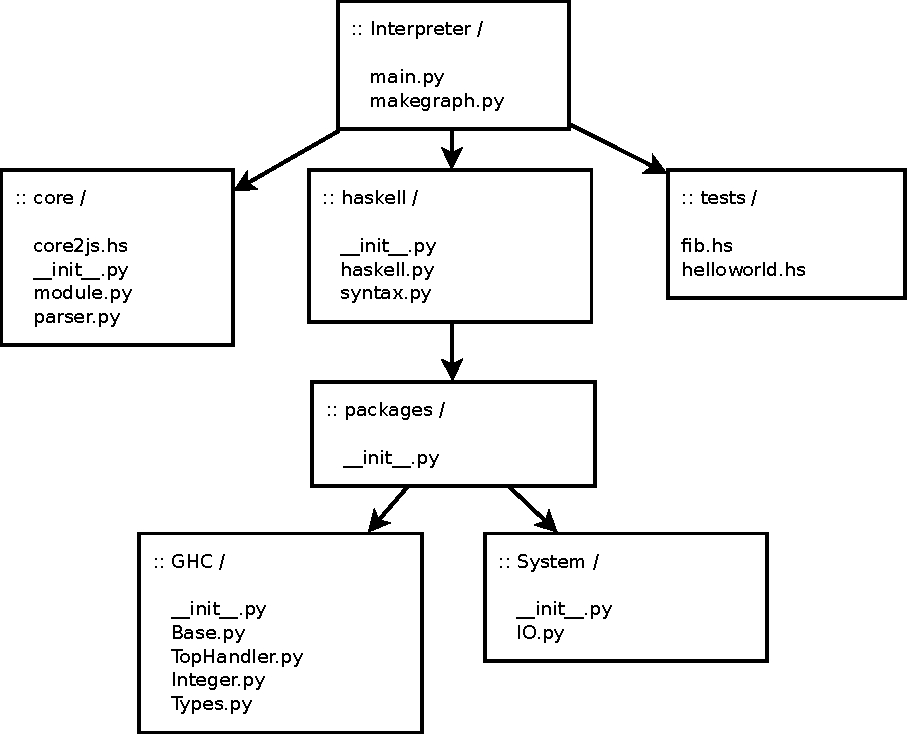
\includegraphics[width=0.8\textwidth]{diags/organization}
\caption{Code tree: The top of the boxes is the folder name, and the rest is the source 
files. Arrows represent subfolders.}
\label{organization}
\end{figure}

\subsection{Serializer}

The serializer consists of two parts; GHC generating external-core, and 
a Haskell program to generate JSCore.

External-core is easily generated by using a compiler flag:
\begin{lstlisting}
ghc -fext-core {path-to-program}
\end{lstlisting}

\begin{figure}[H]
\centering
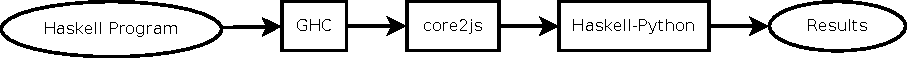
\includegraphics[width=0.8\textwidth]{diags/pipe_w_core2js}
\caption{Pipeline implementation with core2js using extcore}
\label{core2js}
\end{figure}

The Haskell program generating JSCore uses the extcore packages. This package
implements functionality for working with external-core. The result is a datastructure
mapping directly to the external-core format defined in \cite{tolmach2010ghc}. By traversing
this structure, the program builds up a JSON tree using the Haskell JSON package.
The result is a tree of JSON constructs (corresponding to the grammar defined in table \ref{jscore}), 
this is then pretty-printed and dumped to a file.

\subsection{Deserializer}

The deserializer implements a JSON parser. The resulting datastructure is then traversed, building up
an AST using the constructs defined in the Haskell-Python interpreter. 

PyPy implements a parser generator, this simply takes a grammar defined as a string, written in
extended-backus-naur-form (EBNF), and generates a parser. This parser is then used to create a 
JSON datastructure, as represented by table \ref{json}.
The resulting datastructure is then traversed, by checking the contents of the JSON constructs
with the actual external-core format, the Core AST is built. External functionality is imported
as it is encountered. 

After this is done, we are left with a "module" object, corresponding to the initial Haskell
module. 

\subsection{Haskell libraries}

To make some simple test-cases work, some basic Haskell functionality had to be implemented.
Some of this functionality was implemented already in the Haskell-Python Core' interpreter.
The work done here was mostly to organize the functionality into modules corresponding
to Haskell modules. The functionality implemented in these modules does however, not correspond
to the Haskell implementations. This is left for future work, as this is a large task.

From figure \ref{fig:helloworldgraph} (representing a "hello world" program in JSCore), the atomic 
expression "base:SystemziIO.putStrLn" corresponds
to the Haskell function "putStrLn", which is located in the Haskell module "System.IO". This is translated
into a reference to the function "putStrLn" defined in the python module located in 
"haskell/packages/System/IO.py". See figure \ref{organization}.

\subsection{Evaluation}

In order to evaluate the Haskell programs correctly, the expression "main:ZCMain.main" would have
to be reduced to \emph{WHNF}. However, this would require a lot of the functionality used by GHC
to be implemented. Specifically, "GHC.TopHandler.runMainIO()". In order to implement this function
a lot of other functionality would have to be implemented. The function is a wrapper around 
"main:Main.main", it catches uncaught exceptions and flushes stdout/stderr before exiting. 
Implementing this is a goal for further
development, but currently a simple hack is to only evaluate the expression "main:Main.main". This way,
simple programs can be tested by implementing the necessary functionality at a high level, such as the
"putStrLn" function is implemented as a simple "print" function in python.

\subsection{Issues}

\begin{figure}[H]
\centering
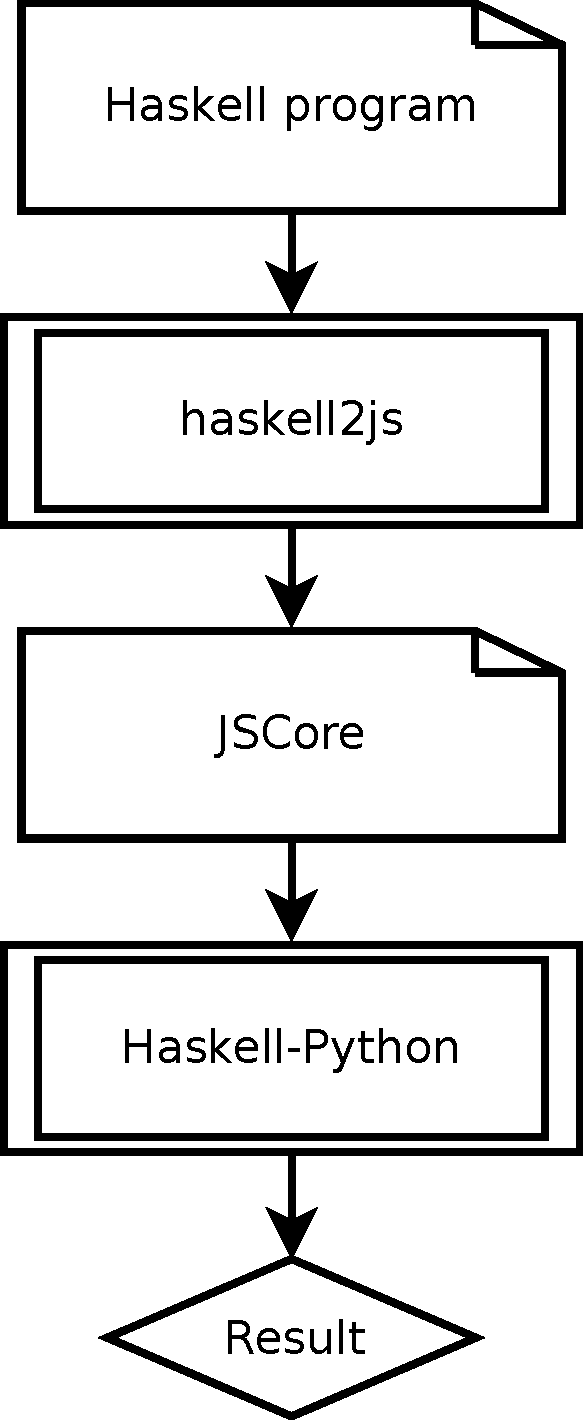
\includegraphics[width=0.8\textwidth]{diags/pipe_w_haskell2js}
\caption{Pipeline with implementation of haskell2js using the GHC API}
\label{haskell2js}
\end{figure}

Very few of the initial plans regarding this project was actually realized in the implementation.
The GHC API was intended to be used to generate JSCore, but this failed do to a lack of experience
with Haskell and the GHC API (see figure \ref{haskell2js} for a description of the initially intended
pipeline). It was then discovered that a lot of the necessary code was already
written in GHC (the code that generates the external-core files), however, this code was not 
exported in any way. It was also deeply embedded in the GHC code. After several attempts at creating
the JSCore format, and some emails back and forth with the GHC team, these methods where abandoned.

The extcore package was then introduced, as it was thought to serve nicely for our purpose. This
does however add an extra step to the generation of JSCore, having to generate external-core
first. There is no way of working with external-core without parsing it from a file. See figure \ref{core2js}.

The reason for not using extcore from the beginning was that it was thought to not be very 
well supported, as the external-core format seems to be changing. This also turned out to be
the case. However, GHC also changes rapidly, and an implementation using the GHC API may not
work for very long either. A version linking to the GHC executable would most likely be the
worst choice.

A large amount of time was spent trying to generate this intermediate format.

The method described here worked well for very trivial Haskell programs, however, it turned out that
the extcore package was not able to parse any nontrivial external-core files generated by GHC versions later 
than 6.10.



% Examples

%\clearpage

\section{Examples}

\lstset{ %
frame=single,                   % adds a frame around the code
tabsize=2,                      % sets default tabsize to 2 spaces
captionpos=b,                   % sets the caption-position to bottom
breaklines=true,                % sets automatic line breaking
}

\subsection{Example 1: hello world}

This example program is a simple "hello world" program, as this was practically
the only program that was able to pass through the entire pipeline. Following
is the "hello world" program written in Haskell:

\begin{footnotesize}
\lstinputlisting[language=Haskell]{"../interpreter/tests/helloworld.hs"}
\end{footnotesize}

\subsubsection{Converted to Core}

After the program has passed through GHC and the external-core file
has been generated, the program looks like this:

\begin{footnotesize}
\lstinputlisting{"../interpreter/tests/helloworld.hcr"}
\end{footnotesize}

... TODO: Explain this representation in more detail.

\subsubsection{Converted to JSCore}

In the next step it is parsed and dumped to JSCore:

\begin{footnotesize}
\lstinputlisting{"../interpreter/tests/helloworld.hcj"}
\end{footnotesize}

\subsubsection{JSCore graph}

Using the parsing libraries of PyPy we can generate a nice graph from the result,
directly corresponding to the resulting datastructure. 
See figure \ref{fig:helloworldgraph}.
By simply traversing this datastructure we can generate the AST for the Core 
interpreter (Haskell-Python).

\begin{sidewaysfigure}
\begin{figure}[H]
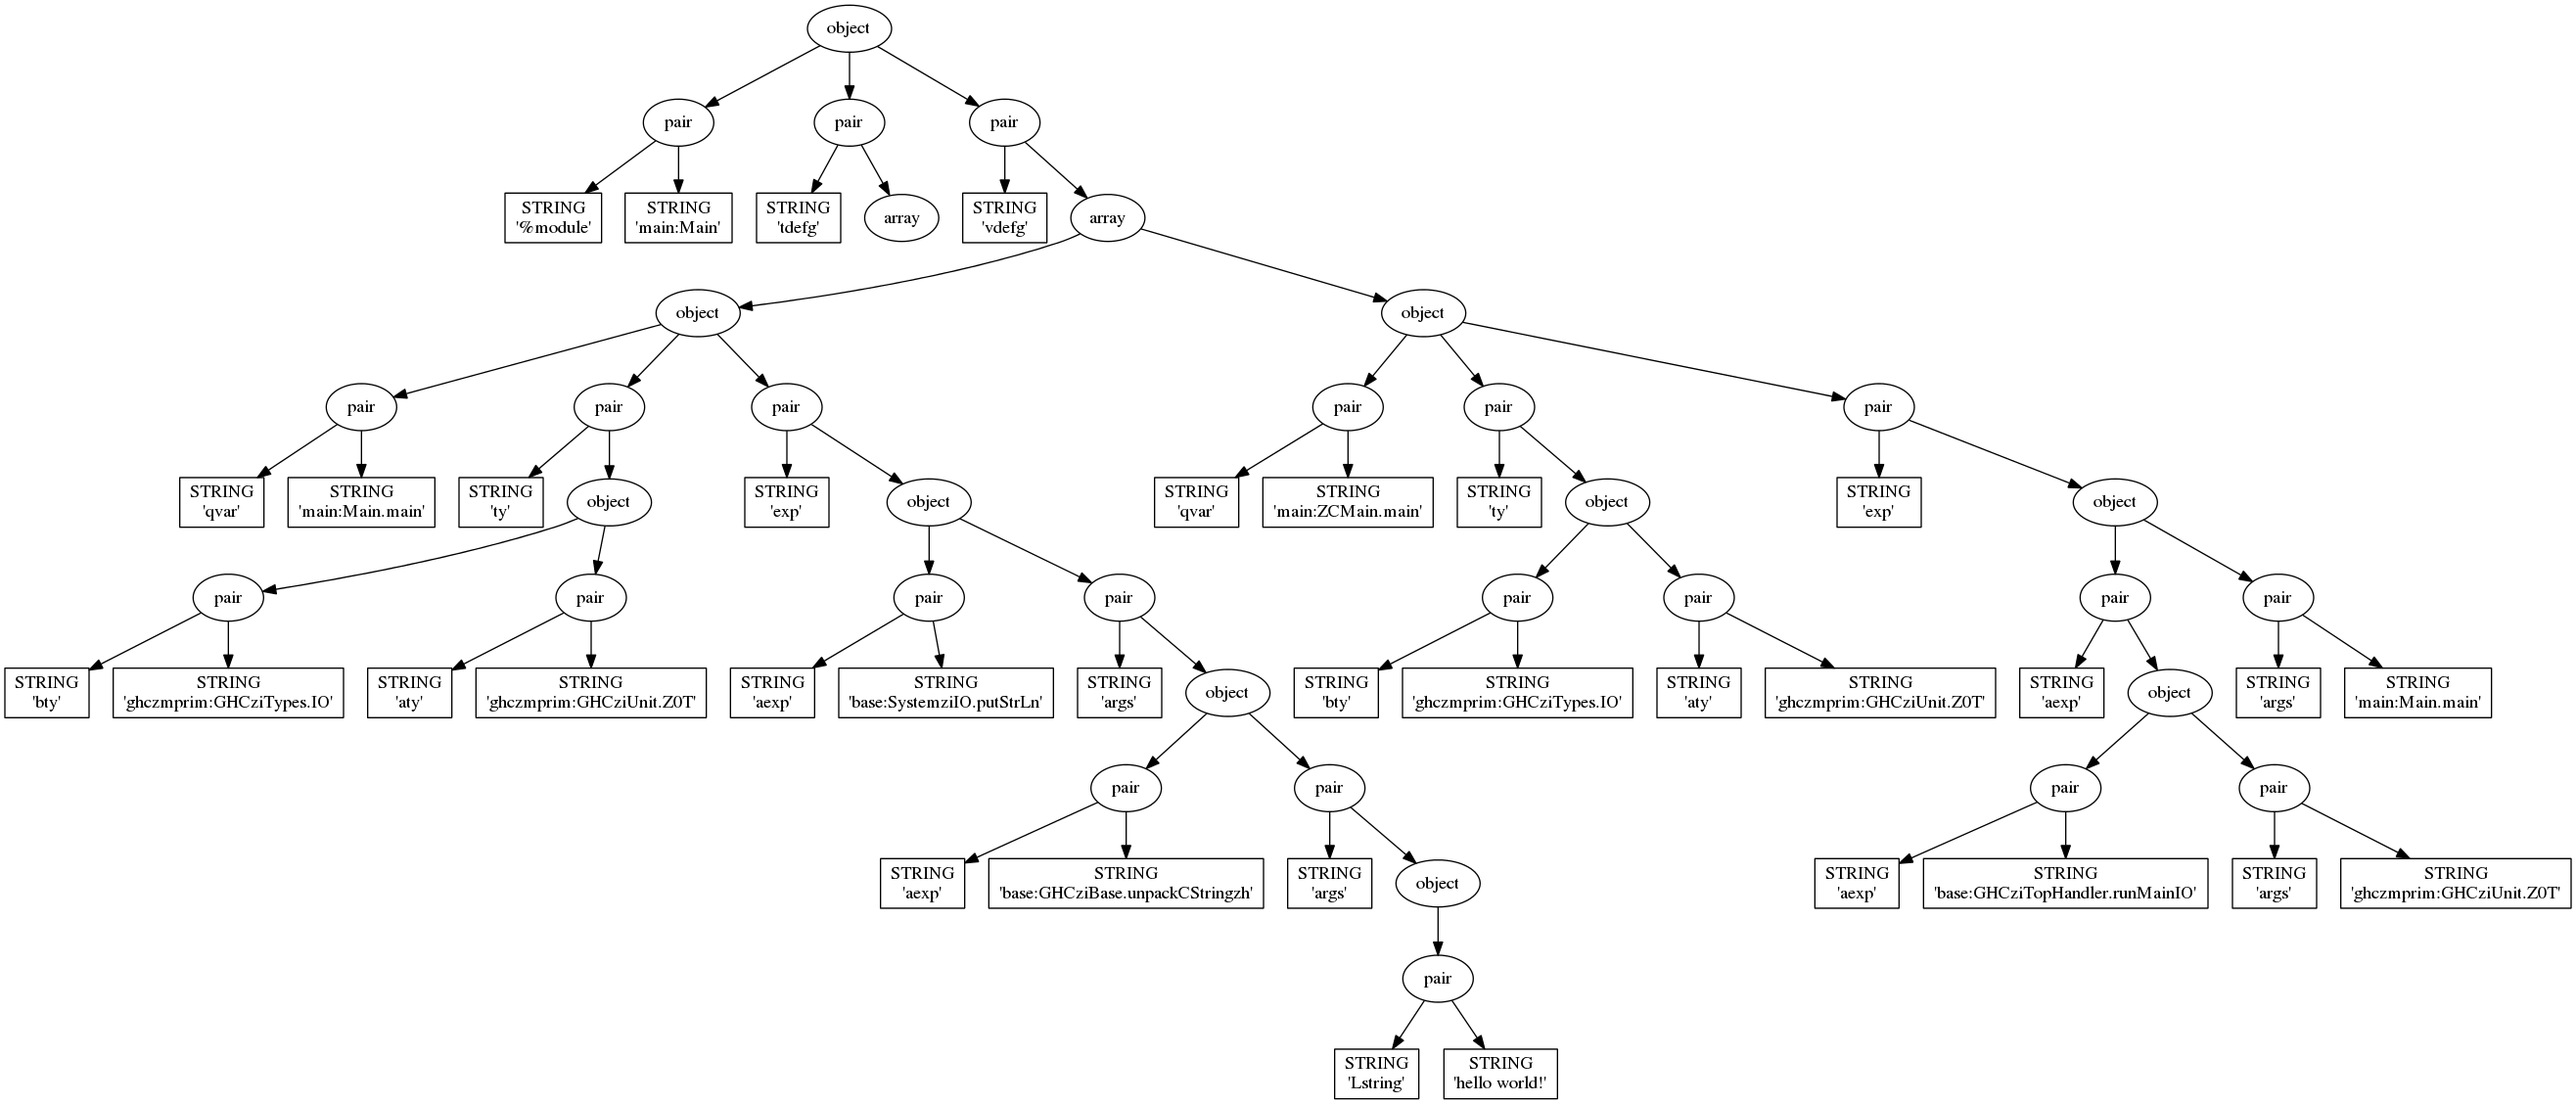
\includegraphics[width=\textwidth]{../interpreter/tests/helloworld.png}
\caption{Example program translated to JSON}
\label{fig:helloworldgraph}
\end{figure}
\end{sidewaysfigure}

\subsubsection{Result}

The program results as expected, outputting the string "Hello, world!".


\subsection{Example 2: naive fibonacci}

The following program is a simple fibonacci program.

\begin{footnotesize}
\lstinputlisting[language=Haskell]{"../interpreter/tests/fib.hs"}
\end{footnotesize}

\subsubsection{Converted to Core}

As we can see, the simple hello world program becomes more complex when translated
to Core by GHC.

\begin{footnotesize}
\lstinputlisting{"../interpreter/tests/fib.hcr"}
\end{footnotesize}

%TODO: Explain this representation in more detail.

\subsubsection{Converted to JSCore}

And translated to JSCore by our serializer:

\begin{footnotesize}
\lstinputlisting{"../interpreter/tests/fib.hcj"}
\end{footnotesize}

\subsubsection{JSCore graph}

Using the parsing libraries of PyPy we can generate a nice graph from the result, 
see figure \ref{fig:fibgraph}

By simply traversing this datastructure we can generate the AST for the Core interpreter.

\begin{sidewaysfigure}
\begin{figure}[H]
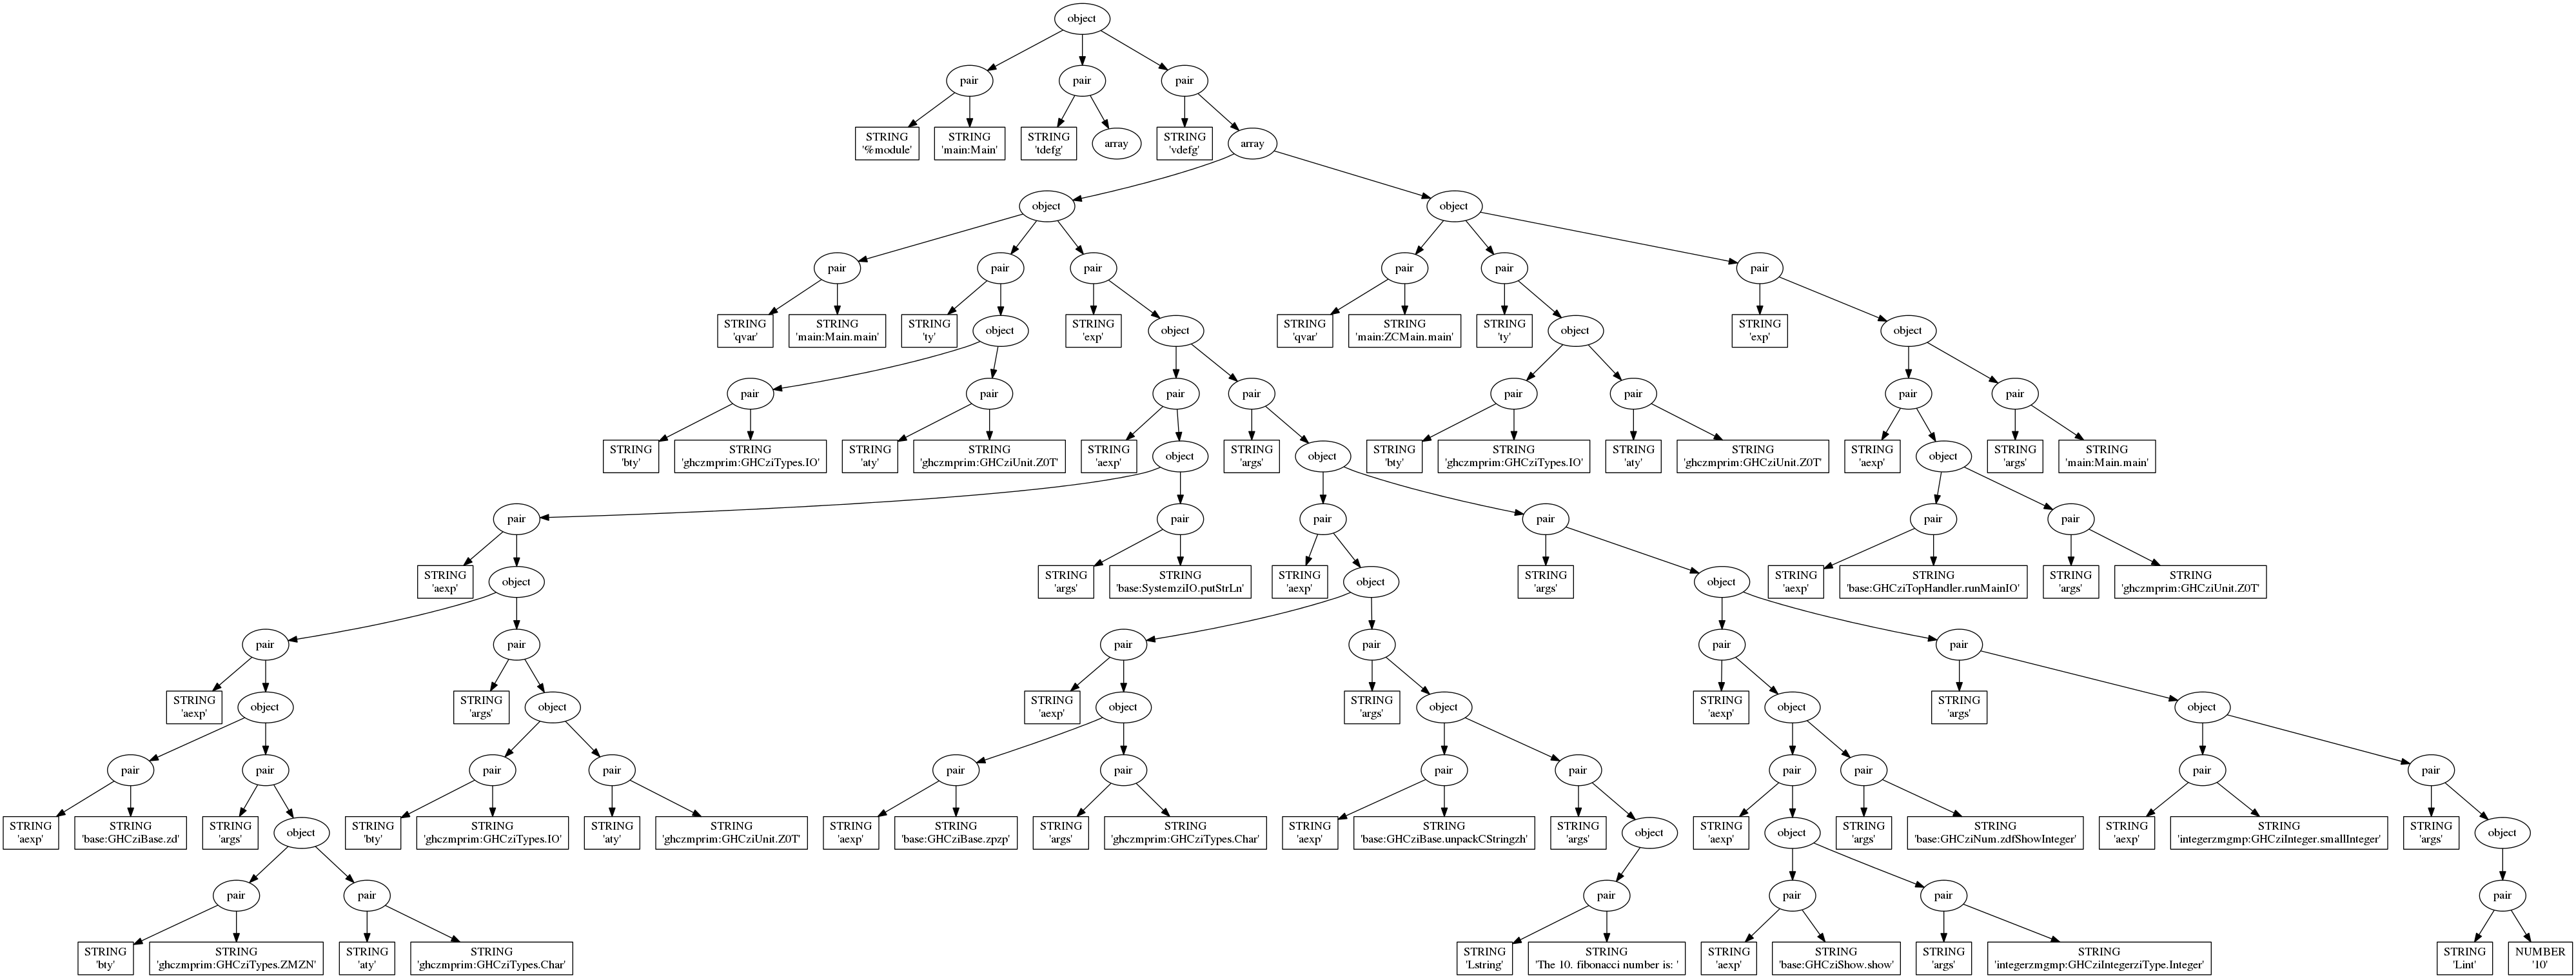
\includegraphics[width=\textwidth]{../interpreter/tests/fib.png}
\caption{Example program 2 translated to JSON}
\label{fig:fibgraph}
\end{figure}
\end{sidewaysfigure}

\subsubsection{Result}



% Future work

%\clearpage
\section{Future work}

\subsection{Getting programs into Haskell-Python from GHC}

This project focused mainly on this task, which was thought to be simple.
However, due to a combination of reasons, this turned out not to be the case.
Mainly, inexperience; with Haskell, the GHC API, and functional languages in 
general. However, a lot of experience was gained during this project, and
future development will benefit from this.

The work involved in this will be revisiting the different possibilities to
achieve our goal. Some options are:

\begin{itemize}
\item Write an external-core parser directly in RPython, and use files generated by GHC.
\item Include development of extcore as a part of the project. This is most likely a bad
idea, as this seems to be no easier than the alternatives.
\item Use the GHC API to generate JSCore, this is also nontrivial.
\item Create functionality to be linked into the GHC executable, in order to generate the
representation of JSCore. Also nontrivial.
\item Simply use the version of GHC matching the version of extcore. This will not be
a good idea for further development of the project, but may be a simple solution to get
a prototype working quickly.
\item Implement a Haskell pipeline in RPython, including parsing, typechecking and desugaring.
This will be a very large task.
\end{itemize}

Either way, understanding of Haskell and Core must be a top priority.

\subsection{Rewrite the deserializer to proper RPython}

The deserializer is currently not written in proper RPython. 
Converting the code to RPython will allow it to be compiled to a JIT interpreter by
the RPython toolchain. This should not be a very big task, but it requires understanding
of the RPython coding style. There are also restrictions on how one may use the PyPy parser
tools.

\subsection{Implement basic Haskell libraries}

Implementing Haskell libraries is necessary to run any Haskell program passed 
through GHC. One option may be to implement (or automatically generate from GHC code) Haskell
primitive types, and to convert the Haskell base libraries to JSCore (or any other format that
may be chosen).

\subsection{Linking functionality}

Currently no thought has been given to the linking between multiple modules. This
must be implemented for any non-trivial Haskell programs to function.

\subsection{Test suite and benchmarking}

A framework for testing and benchmarking should be set up. Allowing us to compare
speed to other implementations, and progress of development. GHC uses a test framework
relying on Python and GNU Make that should be looked into.

\begin{comment}
\subsection{Map GHC encoded Types to Haskell-Python}

Figure out how to create encoded types for Haskell-Python. It may be possible to
autogenerate these from GHC files.

"2.) understanding how GHC encodes types. The Core Haskell of the previous steps encodes the types of all functions in slightly low-level
ways. This needs to be understood and a mapping of these types to what
the Python Haskell interpreter provides needs to be written." 

\subsection{Set up GHC test environment for Haskell-Python}

Setting up the GHC test environment for Haskell-Python would be very valuable
for development and bug fixing.

"3.) the actual interpretation of the Core language is mostly
implemented. There are probably some things missing, which will be
discovered by running some Haskell programs. For that end, it would be
good to find out whether there is a Haskell implementation test suite
and get it to run."

\subsection{Add built in Haskell types to run some Haskell benchmarks}

"4.) what is missing to run more non-pure Haskell programs are all the
built-in functions (e.g. those that perform arithmetic, I/O, call C
functions, etc) and built-in types (e.g. integers, floats, C-level types
like arrays and structs). These should be added step by step. This is an
essentially open-ended task. It would be good to add as many built-ins
so that some of the Haskell benchmarks can run."

\subsection{Optimize PyPy JIT for Haskell-Python}

"5.) JIT work: While the JIT of PyPy can mostly be automatically applied,
in practice a lot of careful work is needed to make sure that the
generated code is optimal (or at least good). To do that, a test suite
of Haskell snippets that explicitly compares the generated machine code
with what it should look like is needed, and then the careful adding of
some tests to this suite, together with the better placement of JIT
hints. This is both the hardest step, as well as the most exciting one."
\end{comment}


% Appendixes
\appendix

% Core grammar
\clearpage
\appendixpage

\section{Formal definition of External-Core}
\label{coregrammar}


The following semantics is used to define the Core grammar, 
as seen in \cite{tolmach2010ghc}:

\begin{scriptsize}

\begin{longtable}{ l c l }

$[$ pat $]$		& :	& optional			\\
$\{$ pat $\}$		& :	& zero or more repetitions	\\
$\{$ pat $\}^{+}$	& :	& one or more repetitions	\\
$pat_{1}|pat_{2}$	& :	& choice			\\

\end{longtable}




\begin{grammar}
<module> ::= \%module <mident> \{ <tdefg> ; \} \{ <vdefg> ; \}
\end{grammar}

\paragraph{Type definitions}

\begin{grammar}
<tdefg> ::= \%data <qtycon> <tbind> = <cdef>
       \alt \%newtype <qtycon> <qtycon> <tbind> = <ty>
\end{grammar}

\paragraph{Constructor definitions}

\begin{grammar}
<cdef> ::= <qdcon> \{ @ <tbind> \} \{ <aty> \}
\end{grammar}

\paragraph{Value definitions}

\begin{grammar}
<vdefg> ::= \%rec \{ <vdef> \{ ; <vdef> \} \}
       \alt <vdef>
\end{grammar}

\begin{grammar}
<vdef> ::= <qvar> :: <ty> = <exp>
\end{grammar}

\paragraph{Atomic Expressions}

\begin{grammar}
<aexp> ::= <qvar>
      \alt <qdcon>
      \alt <lit>
      \alt ( <exp> )
\end{grammar}

\paragraph{Expression}

\begin{grammar}
<exp> ::= <aexp>
     \alt <aexp> \{ <arg> \}
     \alt \textbackslash \{ <binder> \} -$>$ <exp>
     \alt \%let <vdefg> \%in <exp>
     \alt \%case (<aty>) <exp> \%of <vbind> \{<alt> \{ ; <alt> \}  \}
     \alt \%cast <exp> <aty>
     \alt \%note " \{ <char> \} " <exp>
     \alt \%external ccall " \{ <char> " \} <aty>
     \alt \%dynexternal ccall <aty>
     \alt \%label " \{ <char> \} "
\end{grammar}

\paragraph{Argument}

\begin{grammar}
<arg> ::= @ <aty>
     \alt <aexp>
\end{grammar}

\paragraph{Case alternative}

\begin{grammar}
<alt> ::= <qdcon> \{ @ <tbind> \} \{ <vbind> \} -$>$ <exp>
     \alt <lit> -$>$ <exp>
     \alt \%\_ -$>$ <exp>
\end{grammar}

\paragraph{Binder}

\begin{grammar}
<binder> ::= @ <tbind>
        \alt <vbind>
\end{grammar}

\paragraph{Literal}

\begin{grammar}
<lit> ::= ( [-] \{ <digit> \} :: <ty> )
     \alt ( [-] \{ <digit> \} \% \{ <digit> \} :: <ty> )
     \alt ( <char> :: <ty> )
     \alt ( \{ <char> \} )
\end{grammar}

\paragraph{Value binder}

\begin{grammar}
<vbind> ::= ( <var> :: <ty> )
\end{grammar}

\paragraph{Type binder}

\begin{grammar}
<tbind> ::= <tyvar>
       \alt ( tyvar :: <kind> )
\end{grammar}

\paragraph{Atomic type}

\begin{grammar}
<aty> ::= <tyvar>
     \alt <qtycon>
     \alt ( <ty> )
\end{grammar}

\paragraph{Basic type}

\begin{grammar}
<bty> ::= <aty>
     \alt <bty> <aty>
     \alt \%trans <aty> <aty>
     \alt \%sym <aty>
     \alt \%unsafe <aty> <aty>
     \alt \%left <aty>
     \alt \%right <aty>
     \alt \%inst <aty> <aty>
\end{grammar}

\paragraph{Type}

\begin{grammar}
<ty> ::= <bty>
    \alt \%forall \{ <tbind> \} . <ty>
    \alt <bty> -$>$ <ty>
\end{grammar}

\paragraph{Atomic kind}

\begin{grammar}
<akind> ::= *
       \alt \#
       \alt ?
       \alt <bty> :=: <bty>
       \alt ( <kind> )
\end{grammar}

\paragraph{Kind}

\begin{grammar}
<kind> ::= <akind>
      \alt <akind> -$>$ <kind>
\end{grammar}


\paragraph{Names}

\begin{grammar}
<mident>	  ::= 	 '' <pname> : <uname> ''
	
<tycon>		  ::= 	 '' <uname> ''
		
<qtycon>	  ::= 	 '' <mident> . <tycon> ''

<tyvar>		  ::= 	 '' <lname> ''
	
<dcon>		  ::= 	 '' <uname> ''
	
<qdcon>		  ::= 	 '' <mident> . <dcon> ''

<var>		  ::= 	 '' <lname> ''

<qvar>		  ::= 	 '' || <mident> . || <var> ''

<lname>		  ::= 	 <lower> \{ <namechar> \}
 
<uname>		  ::= 	 <upper> \{ <namechar> \}

<pname>		  ::= 	 \{ <namechar> \}$^+$

<namechar>	  ::= 	 <lower> | <upper> | <digit>

<lower>		  ::= 	 a|b|...|z|\_

<upper>		  ::= 	 A|B|...|Z|

<digit>		  ::= 	 0|1|...|9									 


\end{grammar}




\end{scriptsize}


% Z-Encoding
\clearpage
\section{Z-Encoding}
\label{zencoding}

The External-core identifiers are z-encoded. Meaning they use "z" and "Z" as prefixes
for certain symbols:

\begin{tabular}{ | l | l |}
\hline
Character 	& Code	\\
\hline
Tuples:		& 	\\

(\#\#)		& Z1H	\\
()		& Z0T	\\
(,,,)		& Z3T	\\

\hline
Constructors:	&	\\
(		& ZL	\\
)		& ZR	\\
{[}		& ZM	\\
{]}		& ZN	\\
:		& ZC	\\
Z		& ZZ	\\
\hline
Variables:	&	\\
z		& zz	\\	
\&		& za	\\
|		& zb	\\
\^{}		& zc	\\
\$		& zd	\\
=		& ze	\\
>		& zg	\\
\#		& zh	\\
.		& zi	\\
<		& zl	\\
-		& zm	\\
!		& zn	\\
+		& zp	\\
'		& zq	\\
\textbackslash	& zr	\\
/		& zs	\\
{*}		& zt	\\
\_		& zu	\\
\%		& zv	\\
c		& znnnU	\\
\hline
\end{tabular}



% JSON grammar
\clearpage
\section{Formal definition of JSON}
\label{jsongrammar}

\begin{scriptsize}
\begin{longtable}{ r c l r }
\multicolumn{4}{l}{Object}		\\
\\[0.01in]
$object$	& $ \rightarrow $ 	& \{ \}					& \\
 		& $ | $			& \{ $members$ \} 			& \\
$members$ 	& $ \rightarrow $	& $pair$				& \\
		& $ | $			& $pair$ , $members$ 			& \\
$pair$		& $ \rightarrow $	& $string$ : $value$ 			& \\
\\[0.01in]

\multicolumn{4}{l}{Array}		\\
$array$		& $ \rightarrow $	& [ ]					& \\
		& $ | $			& [ $elements$ ]			& \\
$elements$ 	& $ \rightarrow $	& $value$				& \\
		& $ | $			& $value$ , $elements$			& \\
\\[0.01in]

\multicolumn{4}{l}{Value}		\\
$value$		& $ \rightarrow $	& $string$				& \\
		& $ | $			& $number$				& \\
		& $ | $			& $object$				& \\
		& $ | $			& $array$				& \\
		& $ | $			& true					& \\
		& $ | $			& false					& \\
		& $ | $			& null					& \\
\\[0.01in]

\multicolumn{4}{l}{String}		\\
$string$	& $ \rightarrow $	& ""					& \\
		& $ | $			& " $chars$ "				& \\
$chars$		& $ \rightarrow $	& $char$				& \\
		& $ | $			& $char$ $chars$			& \\
$char$		& $ \rightarrow $	& any Unicode character except $"$ 	& \\ 
		&			& or $\backslash$ or control characters: & \\
		&			& $\backslash\backslash$		& \\
		&			& $\backslash /$ 			& \\
		&			& $\backslash b$ 			& \\
		& 			& $\backslash f$ 			& \\
		&			& $\backslash n$			& \\
		& 			& $\backslash r$ 			& \\
		&			& $\backslash t$ 			& \\
		& 			& $\backslash u$ four-hex digits\\
\\[0.01in]

\multicolumn{4}{l}{Number}		\\
$number$	& $ \rightarrow $ 	& $int$ 				& \\
		& $ | $			& $int$ $frac$				& \\
		& $ | $			& $int$ $exp$				& \\
		& $ | $			& $int$ $frac$ $exp$			& \\
$int$		& $ \rightarrow$ 	& $digit$				& \\
		& $ | $ 		& $digit1-9$ $digits$			& \\
		& $ | $ 		& - $digit$				& \\
		& $ | $ 		& - $digit1-9$ $digits$			& \\
$frac$ 		& $ \rightarrow $ 	& . $digits$ 				& \\
$exp$		& $ \rightarrow $ 	& $e$ $digits$ 				& \\
$digits$	& $ \rightarrow $ 	& $digit$				& \\
		& $ | $ 		& $digit$ $digits$			& \\
$e$		& $ \rightarrow $ 	& e					& \\
		& $ | $ 		& e+					& \\
		& $ | $ 		& e- 					& \\
		& $ | $ 		& E					& \\
		& $ | $ 		& E+					& \\
		& $ | $ 		& E-					& \\
\\[0.01in]

\caption{Grammar for JSON}
\label{json}
\end{longtable}

\end{scriptsize}




% JSCore grammar
\clearpage

\chapter{Formal definition of JSCore}
\label{jscoregrammar}


\begin{grammar}
<module> 	::= \{ ''\%module'' : <mident> , ''tdefg'' : [ <tdefg> ] , ''vdefg'' : [ <vdefg> ] \}
\end{grammar}

\paragraph{Type definitions}

\begin{grammar}
<tdefg> 	  ::= 	 \{ ''\%data'' : <qtycon> , ''tbind'' : [ <tbind> ], ''cdef'' : [ <cdef> ] \}						
		  \alt 	 \{ ''\%newtype'' : <qtycon> , ''qtycon'' : <qtycon> , ''tbind'' : [ <tbind> ] , ''ty'' : <ty> \} 	

\end{grammar}

\paragraph{Constructor definitions}

\begin{grammar}


<cdef>		  ::= 	 \{ ''qdcon'' : <qdcon> , ''tbind'' : [ <tbind>  ] , ''aty'' : [<aty>]$^{+}$ \} 				 			

\end{grammar}

\paragraph{Value definitions}

\begin{grammar}

<vdefg>		  ::= 	\{ ''\%rec'' : [ <vdef> ]$^{+}$ \}    							
		  \alt 	<vdef>
<vdef> 		  ::= 	\{ ''qvar'' : <qvar> , ''ty'' : <ty> , ''exp'' : <exp> \}

\end{grammar}

\paragraph{Atomic Expressions}
\begin{grammar}


<aexp>		  ::= 	 \{ ''qvar'' : <qvar> \}
		  \alt 	 \{ ''qdcon'' : <qdcon> \}
		  \alt 	 \{ ''lit'' : <lit> \}
		  \alt 	 \{ ''exp'' : <exp> \} 


\end{grammar}

\paragraph{Expressions}

\begin{grammar}

<exp>		  ::= 	 <aexp>
		  \alt 	 \{ ''aexp'' : <aexp> , ''args'' : [ <arg> ]$^{+}$ \} 				
		  \alt 	 \{ ''lambda'' : [ <binder> ] , ''exp'' : <exp> \}		
		  \alt 	 \{ ''\%let'' : <vdefg> , ''\%in'' : <exp> \}				
		  \alt 	 \{ ''\%case'' : <aty> , ''exp'' : <exp> , ''\%of'' : <vbind>, ''alt'' : [ <alt> ]$^{+}$ \}	
		  \alt 	 \{ ''\%cast'' : <exp> , ''aty'' : <aty>	\}		
		  \alt 	 \{ ''\%note'' : ''  \{ <char> \} '' , ''exp'' : <exp>	\}	
		  \alt 	 \{ ''\%external ccal'' : '' \{ <char> \} '' , ''aty'' : <aty> \}	
		  \alt 	 \{ ''\%dynexternal ccal'' : <aty> \}
		  \alt 	 \{ ''\%label'' : '' \{ <char> \} '' \}


\end{grammar}

\paragraph{Argument}

\begin{grammar}

<arg>		  ::= 	 \{ ''aty'' : <aty> \}											 
		  \alt 	 \{ ''aexp'' : <aexp> \}										


\end{grammar}

\paragraph{Case alternative}
\begin{grammar}

<alt>		  ::= 	 \{ ''qdcon'' : <qdcon> , ''tbind'' : [ <tbind> ] , ''vbind'' : [ <vbind> ] , ''exp'' : <exp> \}
		  \alt 			 \{ ''lit'' : <lit> , ''exp'' : <exp> \}
		  \alt 			 \{ ''\%\_'' : <exp> \}	


\end{grammar}

\paragraph{Binder}

\begin{grammar}

<binder>	  ::= 	\{ ''tbind'' : <tbind> \}		
		  \alt 	\{ ''vbind'' : <vbind> \}	


\end{grammar}

\paragraph{Type binder}

\begin{grammar}

<tbind>		  ::= 	 \{ ''tyvar'' : <tyvar> \}
		  \alt 	 \{ ''tyvar'' : <tyvar> , ''kind'' : <kind> \}	


\end{grammar}

\paragraph{Value binder}

\begin{grammar}

<vbind>		  ::= 	 \{ ''var'' : <var> , ''ty'' <ty> \} 										 

\end{grammar}

\paragraph{Literal}

\begin{grammar}


<lit>		  ::= 	<jsstring>		 
		  \alt 	<jsnumber>


<jsstring>	  ::= 	 ''''														 
		  \alt 	'' <jschars> ''		
											 
<jschars>	  ::= 	<jschar>
		  \alt 	<jschar> <jschars>
												 
<jschar>	  ::= 	 See definition below

<jsnumber>	  ::=  	<jsint>
		  \alt 	<jsint> <jsfrac>
		  \alt 	<jsint> <jsexp>
		  \alt 	<jsint> <jsfrac> <jsexp>
											 
<jsint>		  ::= 	<jsdigit>
		  \alt  <jsdigit1-9> <jsdigits> 
		  \alt  - <jsdigit>
		  \alt  - <jsdigit1-9> <jsdigits>

<jsfrac> 	  ::=  	. <jsdigits>

<jsexp>		  ::=  	<jse> <jsdigits>

<jsdigits>	  ::=  	<jsdigit> 
		  \alt  <jsdigit> <jsdigits>

<jse>		  ::=  	e
		  \alt  e+		 
		  \alt  e- 		 
		  \alt  E		 
		  \alt  E+		 
		  \alt  E-

\end{grammar}

\paragraph{Atomic Type}

\begin{grammar}
<aty>		  ::= 	 \{ ''tyvar'' : <tyvar> \}
		  \alt 	 \{ ''qtycon'' : <qtycon> \}
		  \alt   \{ ''ty'' : <ty> \}

\end{grammar}

\paragraph{Basic Type}

\begin{grammar}
<bty>		  ::= 	 <aty>
		  \alt 	 \{ ''bty'' : <bty> , ''aty'' , <aty> \}
		  \alt 	 \{ ''\%trans'' : <aty> , ''aty'' : <aty> \}
		  \alt 	 \{ ''\%sym'' : <aty> \}
		  \alt 	 \{ ''\%unsafe'' : <aty> , ''aty'' : <aty> \}	
		  \alt 	 \{ ''\%left'' : <aty> \}
		  \alt 	 \{ ''\%right'' : <aty> \}	
		  \alt 	 \{ ''\%inst'' : <aty> , ''aty'' : <aty> \}


\end{grammar}

\paragraph{Type}

\begin{grammar}

<ty>		  ::= 	 <bty>
		  \alt 	 \{ ''\%forall'' :  [ <tbind> ]$^+$ , ''ty'' : <ty> \}	
		  \alt 	 \{ ''bty'' <bty> , ''ty'' : <ty> \} 


\end{grammar}

\paragraph{Atomic Kind}

\begin{grammar}

<akind>		  ::= 	 *	
		  \alt 	 \#
		  \alt 	 ?	
		  \alt 	 \{ ''bty'' : <bty< , ''bty'' : <bty> \}
		  \alt 	 \{ ''kind'' : <kind> \}	


\end{grammar}

\paragraph{Kind}

\begin{grammar}

<kind>		  ::= 	\{ ''akind'' : <akind> \}					
		  \alt 	\{ ''akind'' : <akind> , ''kind'' : <kind> \}		

<mident>	  ::= 	 '' <pname> : <uname> ''
	
<tycon>		  ::= 	 '' <uname> ''
		
<qtycon>	  ::= 	 '' <mident> . <tycon> ''

<tyvar>		  ::= 	 '' <lname> ''
	
<dcon>		  ::= 	 '' <uname> ''
	
<qdcon>		  ::= 	 '' <mident> . <dcon> ''

<var>		  ::= 	 '' <lname> ''

<qvar>		  ::= 	 '' || <mident> . || <var> ''

<lname>		  ::= 	 <lower> \{ <namechar> \}
 
<uname>		  ::= 	 <upper> \{ <namechar> \}

<pname>		  ::= 	 \{ <namechar> \}$^+$

<namechar>	  ::= 	 <lower> | <upper> | <digit>

<lower>		  ::= 	 a|b|...|z|\_

<upper>		  ::= 	 A|B|...|Z|

<digit>		  ::= 	 0|1|...|9									 


\end{grammar}




% Test programs
\clearpage
\section{Test programs}
\label{testprograms}

\subsection{helloworld}

\lstinputlisting[language=Haskell]{"../interpreter/tests/helloworld/helloworld.hs"}

\subsection{helloworld2}

\lstinputlisting[language=Haskell]{"../interpreter/tests/helloworld2/helloworld2.hs"}

\subsection{factorial}

\lstinputlisting[language=Haskell]{"../interpreter/tests/factorial/factorial.hs"}

\subsection{fibonacci}

\lstinputlisting[language=Haskell]{"../interpreter/tests/fibonacci/fibonacci.hs"}




% JSCore program graphs
%\clearpage
%\section{Graphs of programs in JSCore}
\label{graphs}

\begin{sidewaysfigure}
\begin{figure}[H]
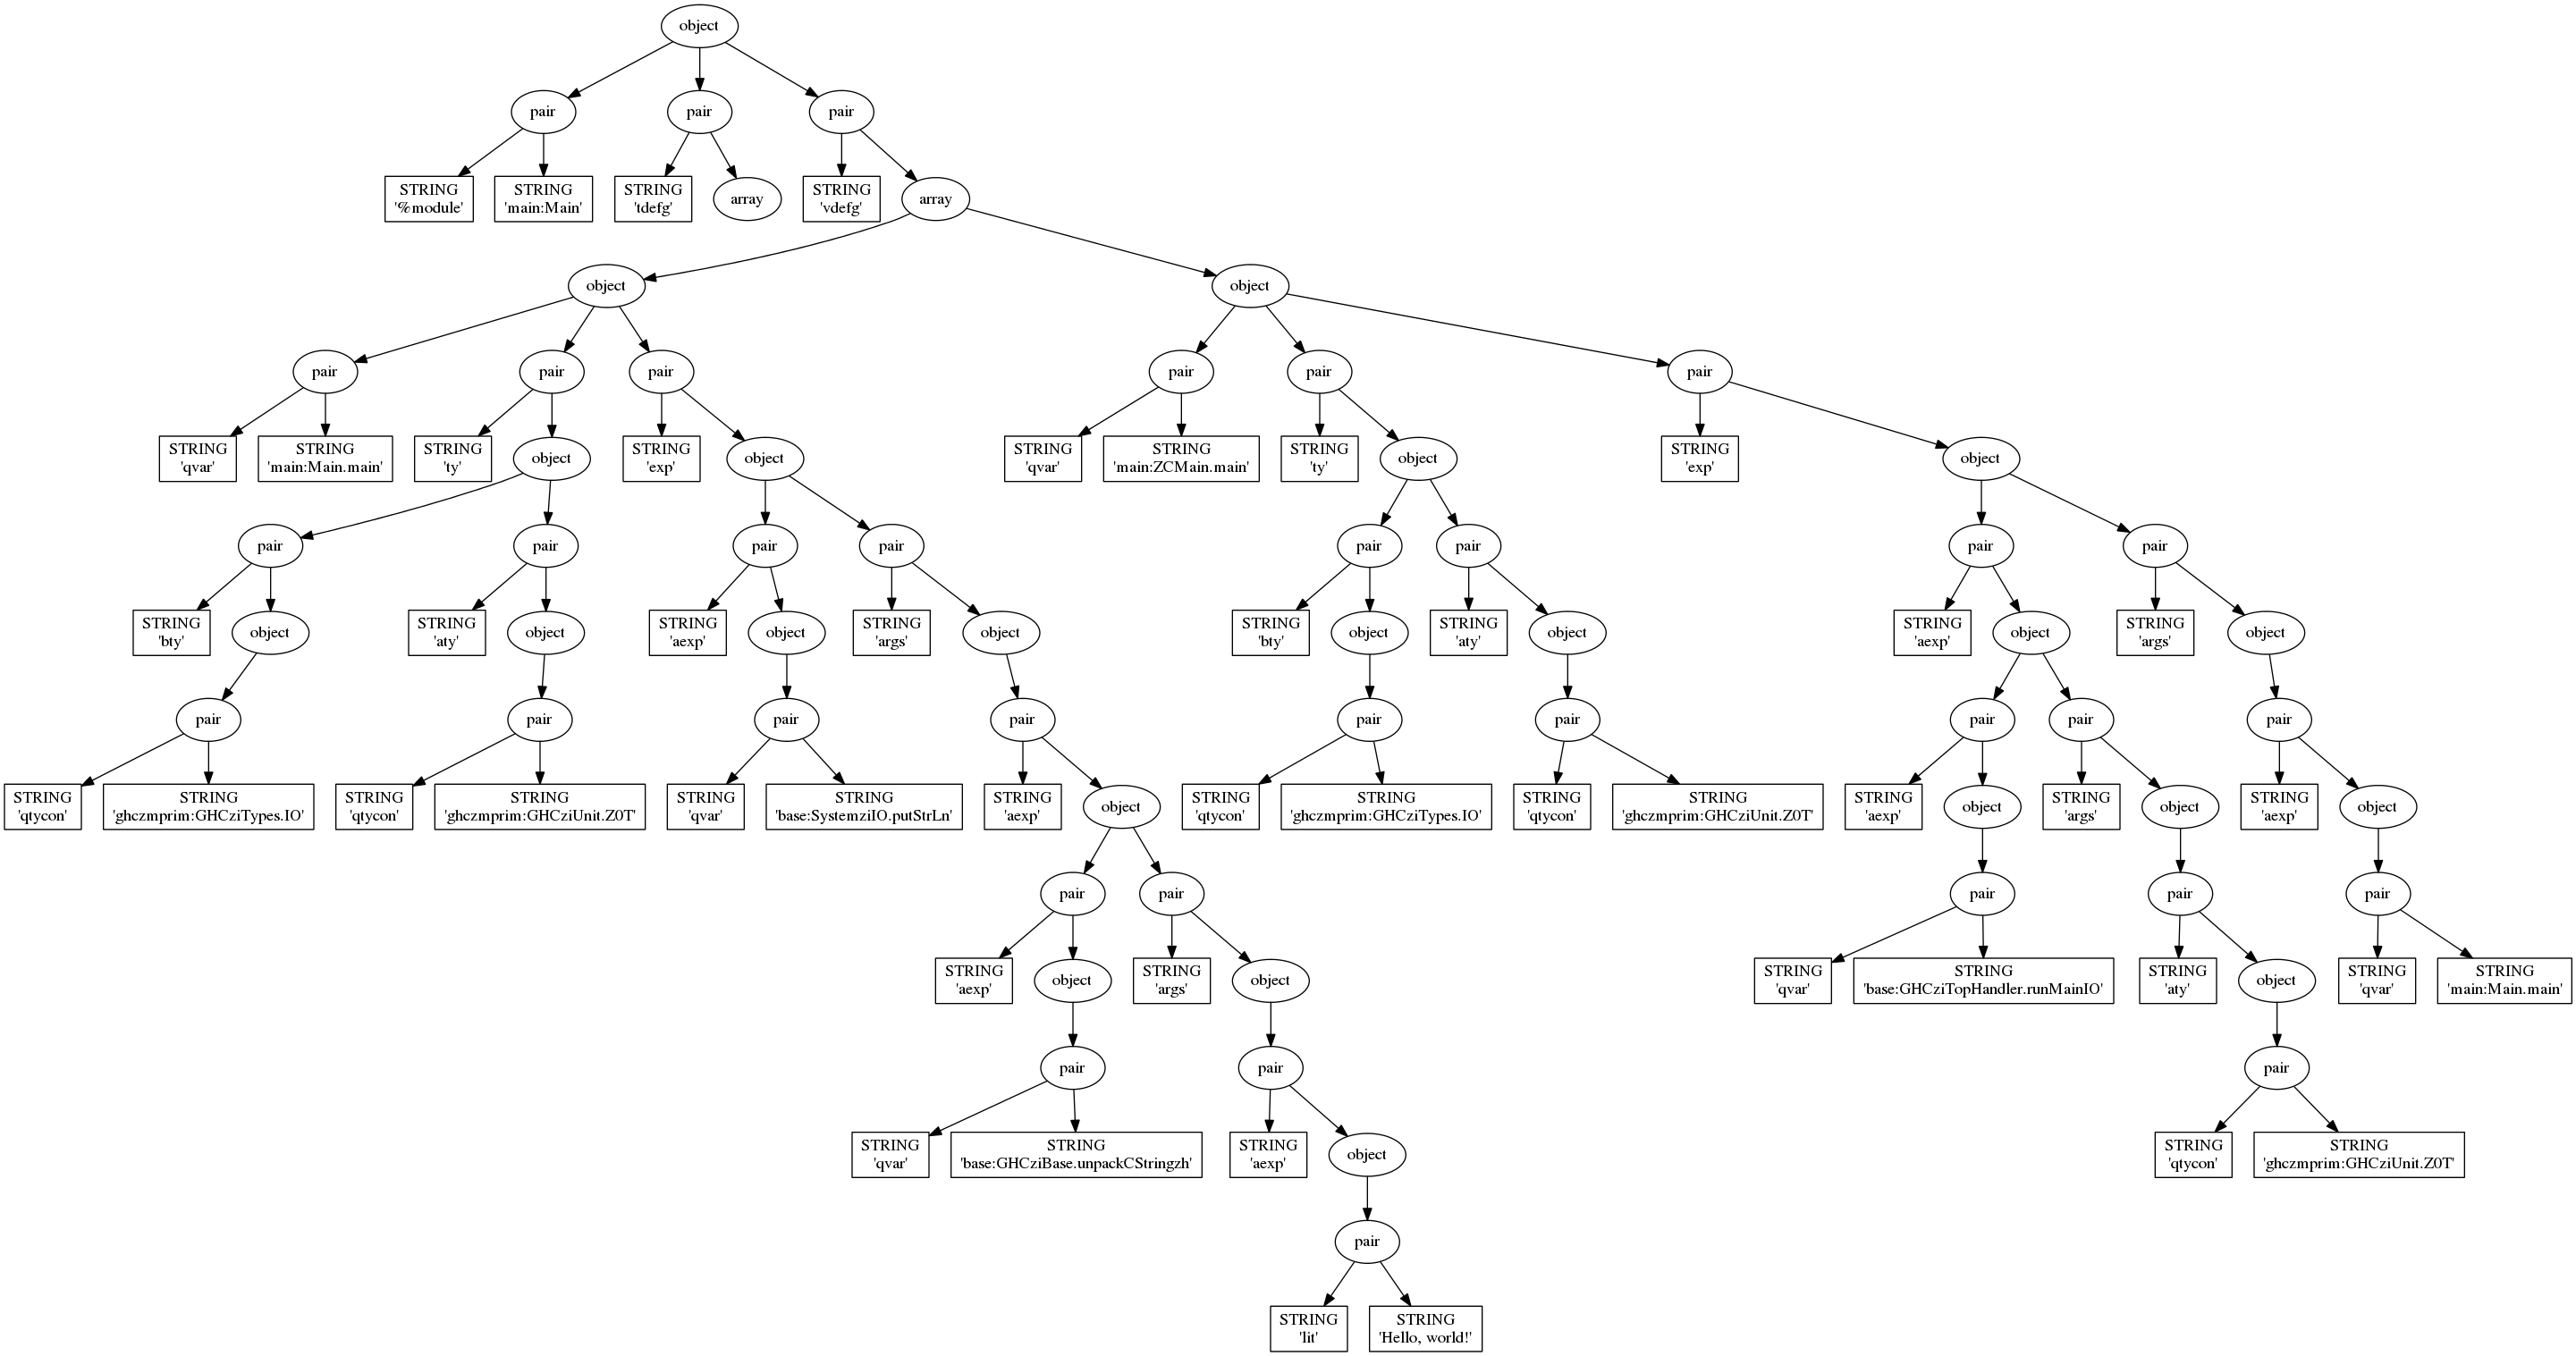
\includegraphics[width=\textwidth]{../interpreter/tests/helloworld/helloworld.png}
\caption{Example program translated to JSCore}
\label{helloworldgraph}
\end{figure}
\end{sidewaysfigure}

\begin{comment}

\begin{sidewaysfigure}
\begin{figure}[H]
\includegraphics[width=\textwidth]{../interpreter/tests/factorial/factorial.png}
\caption{Example program translated to JSCore}
\label{helloworldgraph}
\end{figure}
\end{sidewaysfigure}

\end{comment}


% References
\clearpage
\bibliographystyle{plain}
\bibliography{papers}

\end{document}
